\documentclass[utf8]{book}
\def\allfiles{}
\usepackage{titletoc}
\usepackage{titlesec}
\usepackage{ctexcap}
\usepackage[b5paper,text={125mm,195mm},centering,left=1in,right=1in,top=1in,bottom=1in]{geometry}
\usepackage[]{geometry}
\usepackage{imakeidx}
\usepackage{multicol}
\usepackage{hyperref}
\usepackage{caption}
\usepackage{graphicx, subfig}
\usepackage{amsmath}
\usepackage{xcolor}
\usepackage{listings}
\lstset{%
	breaklines=true,
	tabsize=2
}
\newcommand\Emph{\textbf}
\makeindex
\bibliographystyle{plain}
\begin{document}
\title{\heiti 以太坊学习}
\author{\fangsong 邹远春}
\date{2018年6月}

\frontmatter
\maketitle

\chapter{序 I}

以太坊作为智能合约2.0的鼻祖,学习它有助于了解区块链。

\chapter{序 II}

学习以太坊之后,了解DAPP,解放生产生产关系,促进生产力的提升。

\chapter{前~言}

以太坊在区块链历史上具有划时代的意义,图灵完备的智能合约,打开了一扇DAPP大门,重构整个社会商业模式。

\renewcommand\contentsname{目~录}
\tableofcontents

\mainmatter

\part{理论基础}

\ifx\allfiles\undefined
\documentclass[UTF8]{ctexart}
\title{密码学安全}
\author{邹远春}
\date{}
\usepackage{xeCJK}
\usepackage{graphicx}
\usepackage{listings}
\usepackage{verbatim}
\begin{document}
\maketitle
\else
\chapter{密码学安全}
\fi
\section{公钥密码学}

\subsection{RSA}

\subsection{离散对数ElGamal}

\subsection{椭圆曲线密码学ECC}

\subsection{数字签名}

\subsubsection{Schnorr}

\subsubsection{Secp256k1}

[以太坊源代码分析] IV. 椭圆曲线密码学和以太坊中的椭圆曲线数字签名算法应用
https://blog.csdn.net/teaspring/article/details/77834360

\section{哈希}

\paragraph{SHA-3哈希加密}
SHA-3在2015年8月由美国标准技术协会(NIST)正式发布,作为Secure Hash Algorithm家族的最新一代标准。

\section{安全多方计算}

\subsection{保护隐私的电子投票协议}

\section{比特承诺}

\section{高级签名协议}

\subsection{盲签名}

\subsection{环签名}

\section{零知识证明}

\subsection{$\sum$协议}

\subsection{Bulletproofs}

\subsection{zkSnarks}

\subsection{zkStarks}

\section{秘密分享与门限密码学}

\subsection{密码分享}

\subsubsection{VSS}

\subsubsection{基于VSS的随机数生成}

\subsection{门限密码}

\subsection{门限签名}

\subsubsection{BLS}

\section{量子安全}

%\begin{multicols}{2}
%清朝中期, 外国人就开始中国采集植物标本。清朝中期, 外国人就开始中国采集植物标本。清朝中期, 外国人就开始中国采集植物标本。清朝中期, 外国人就开始中国采%集植物标本。清朝中期, 外国人就开始中国采集植物标本。清朝中期, 外国人就开始中国采集植物标本。
%\end{multicols}
\ifx\allfiles\undefined
\end{document}
\fi %密码学安全

\ifx\allfiles\undefined
\documentclass[UTF8]{ctexart}
\title{共识算法}
\author{邹远春}
\date{}
\usepackage{xeCJK}
\usepackage{graphicx}
\usepackage{listings}
\usepackage{verbatim}
\begin{document}
\maketitle
\else
\chapter{共识算法}
\fi
\section{PoW}

这一系列有很多共识算法。

\subsection{SHA256}

\subsubsection{Bitcoin}

\subsection{Ethan}

\subsubsection{ETH}

\subsection{Scrypt}

\subsubsection{Litecoin}

后期列出门罗、Zcash等等项目的共识算法

\section{PoS}

\subsection{Casper}

\subsection{Tendermint}

\subsection{Qtum}

\subsection{BlackCoin}

\section{DPoS}

\subsection{EOS}

\subsection{ACT}

\section{PBFT}

\subsection{NEO}

\subsection{Tendermint}

\section{VRF}

\subsection{Dfinity}

\subsection{ONT}

\section{人工智能}

\subsection{BTM}

\section{DAG}

\subsection{IOTA}

\subsection{PHANTOM}

DAG区块链项目SPECTRE

\subsection{Hashgraph}

哈希图

\ifx\allfiles\undefined
\end{document}
\fi %共识算法

\ifx\allfiles\undefined
\documentclass[UTF8]{ctexart}
\title{知识准备}
\author{邹远春}
\date{}
\usepackage{xeCJK}
\usepackage{graphicx, subfig}
\usepackage{caption}
\usepackage{listings}
\usepackage{verbatim}
\begin{document}
\maketitle
\else
\chapter{知识准备}
\fi
\section{RLP}

https://github.com/ethereum/wiki/wiki/RLP

\subsection{Definition}

\subsection{Examples}

\subsection{RLP~decoding}

\section{MPT}

以太坊MPT详解

https://blog.csdn.net/weixin\_41545330/article/details/79370198

\begin{figure}
	\centering
	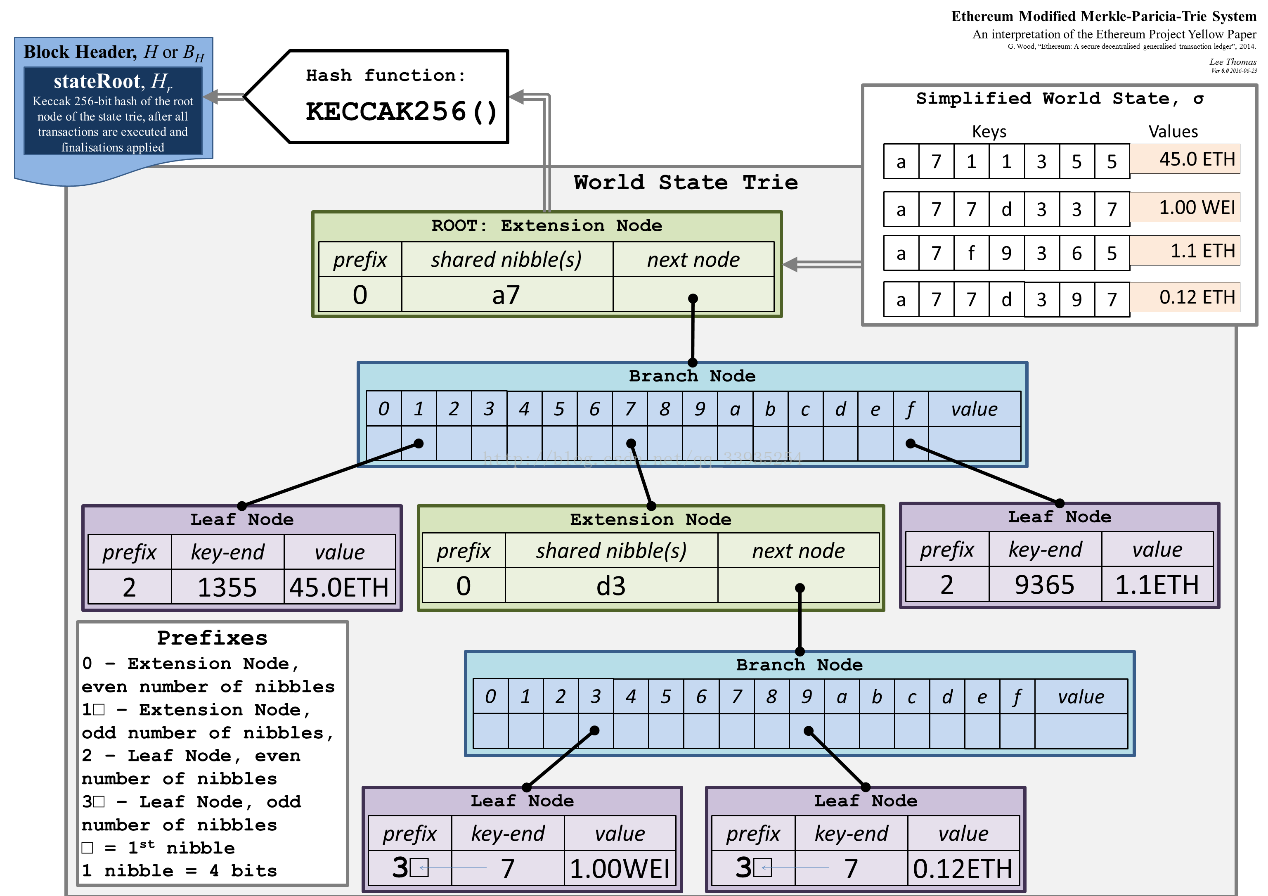
\includegraphics{rlp.png}
	\caption{MTP}
	\label{rlp}
\end{figure}

\section{矿池}

\section{矿机}

\section{世界状态}

\section{分叉}

\section{侧链}

RootStock

\section{闪电网络}

\section{隔离见证}

\section{智能合约}

\section{跨链}

\subsection{公证人}
Notary schemes

\subsection{侧链/中继}
Sidechains/relays

BTC-Replay

Cosmos

Polkadot

\subsection{哈希锁定}
Hash-locking

HTLC

\section{预言机Oracle}

\section{Sharding}

\section{中心化交易所}

\section{去中心化交易所}

\section{钱包}

\subsection{热钱包}

\subsection{冷钱包}

\subsection{硬件钱包}

\subsection{分层确定性钱包}

\section{ERC20}

\section{ERC721}

\section{安全}
形式化证明

\ifx\allfiles\undefined
\end{document}
\fi %知识准备

\part{源码学习}

\ifx\allfiles\undefined
\documentclass[UTF8]{ctexart}
\title{以太坊架构设计}
\author{邹远春}
\date{}
\usepackage{xeCJK}
\usepackage{graphicx}
\usepackage{listings}
\usepackage{verbatim}
\begin{document}
\maketitle
\else
\chapter{以太坊架构设计}
\fi
\section{核心概念}

\paragraph{EVM}
以太坊虚拟机,轻量级的虚拟机环境,是以太坊智能合约的执行环境。

\paragraph{Account}

账户分为合约账户和外部账户。合约账户主要存储执行的合约代码;外部账户对应用户账户。

\paragraph{Transaction}

以太坊网络上的交易,从一个账户到另一个账户的消息,包括以太币或智能合约参数。

\paragraph{Gas}

以太坊执行智能合约的燃料。

\paragraph{Miner}
挖矿,以太坊网络通过共识算法来保证网络的安全运行。

\paragraph{P2P网络通信}
以太坊分布式网络中所有节点地位平等,没有中心化服务器。

\section{架构设计}

椭圆曲线数字签名Secp256k1

梅克尔树链式存储

MTP(Merkle Patricia Trie)

账户交易模型

LevelDB数据存储

P2P网络通信

Ethan/Casper共识算法

挖矿激励

图灵完备的智能合约执行环境EVM

\section{源码目录结构}

\paragraph{accounts}
以太坊账户管理

\paragraph{bmt}
二进制MPT的实现

\paragraph{build}
主要是一些编译和构建的脚本与配置

\paragraph{cmd}
命令行工具

\subparagraph{abigen} 合约接口生成工具
\subparagraph{bootnode}实现网络发现的节点
\subparagraph{clef}
\subparagraph{ethkey}
\subparagraph{evm} 以太坊虚拟机
\subparagraph{faucet}
\subparagraph{geth} 以太坊命令行客户端
\subparagraph{intrnal}
\subparagraph{p2psim}
\subparagraph{puppeth} 创建一个新的以太坊网络的向导
\subparagraph{rlpdump} 提供RLP数据的格式化输出
\subparagraph{swarm} swarm网络的接入点
\subparagraph{utils} 公共的组件
\subparagraph{wnode} 这是一个简单的Whisper节点。 它可以用作独立的引导节点。此外,可以用于不同的测试和诊断目的。

\paragraph{common} 一些公共的工具类
\paragraph{consensus} 共识算法
\paragraph{console}
\paragraph{containers}
\paragraph{contracts}
\paragraph{core} 核心数据结构与算法
\paragraph{crypto} 加密、数字签名和哈希算法
\paragraph{dashboard}
\paragraph{eth} 实现以太坊协议
\paragraph{ethclient} 以太坊RPC客户端
\paragraph{ethdb} 以太坊数据库,主要是LevelDB相关接口
\paragraph{ethstats}
\paragraph{event} 事件处理
\paragraph{internal}
\paragraph{les}
\paragraph{light} 实现为以太坊轻量级客户端提供按需检索的功能
\paragraph{log}
\paragraph{metrics} 提供磁盘计数器
\paragraph{miner} 挖矿
\paragraph{mobile} 移动端
\paragraph{node} 多种类型的节点
\paragraph{p2p} p2p网络通信
\paragraph{params}
\paragraph{rlp} 以太坊序列化和反序列化
\paragraph{rpc} 远程方法调用
\paragraph{signer}
\paragraph{swarm} swarm网络处理
\paragraph{tests}
\paragraph{trie} MPT实现
\paragraph{vendor}
\paragraph{whisper}  whisper节点协议
\ifx\allfiles\undefined
\end{document}
\fi % 以太坊架构设计

\ifx\allfiles\undefined
\documentclass[UTF8]{ctexart}
\title{以太坊启动、合约与交易}
\author{邹远春}
\date{}
\usepackage{xeCJK}
\usepackage{graphicx}
\usepackage{listings}
\usepackage{verbatim}
\usepackage{graphicx}
\usepackage{xcolor}
\usepackage{listings}
\lstset{%
	breaklines=true,
	tabsize=2
}
\begin{document}
\maketitle
\newcommand\Emph{\textbf}
\else
\chapter{以太坊}
\fi
\section{以太坊启动}

\subsection{源码}

\subsection{私有链搭建}

\section{EVM执行分析}

\section{区块数据结构}

\begin{figure}
	\centering
	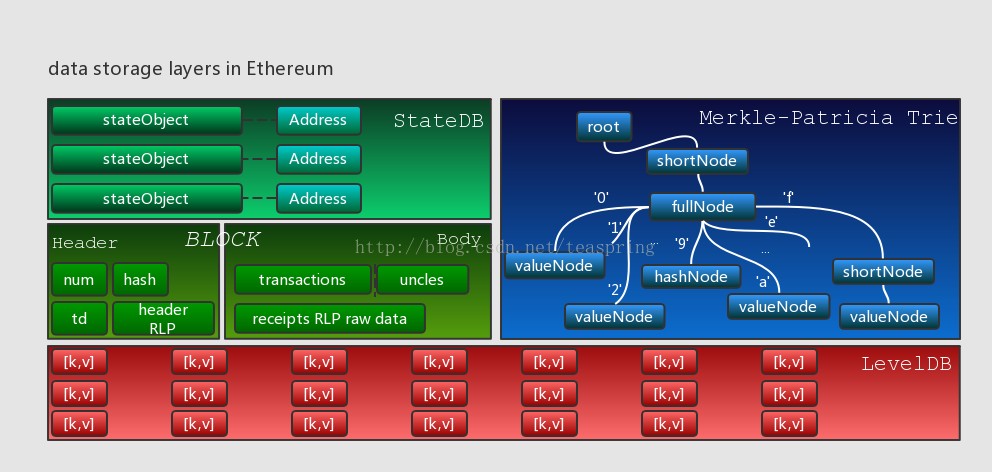
\includegraphics[scale=0.45]{data_storage.png}
	\caption{data storage layers in Ethereum}
	\label{dataStorage}
\end{figure}

\subsection{Block和Header}

Block(区块)是Ethereum的核心数据结构之一。所有账户的相关活动,以交易(Transaction)的格式存储,每个Block有一个交易对象的列表;每个交易的执行结果,由一个Receipt对象与其包含的一组Log对象记录;所有交易执行完后生成的Receipt列表,存储在Block中(经过压缩加密)。不同Block之间,通过前向指针ParentHash一个一个串联起来成为一个单向链表,BlockChain 结构体管理着这个链表。

Block结构体基本可分为Header和Body两个部分,其UML关系族如下图所示:


\begin{figure}
	\centering
	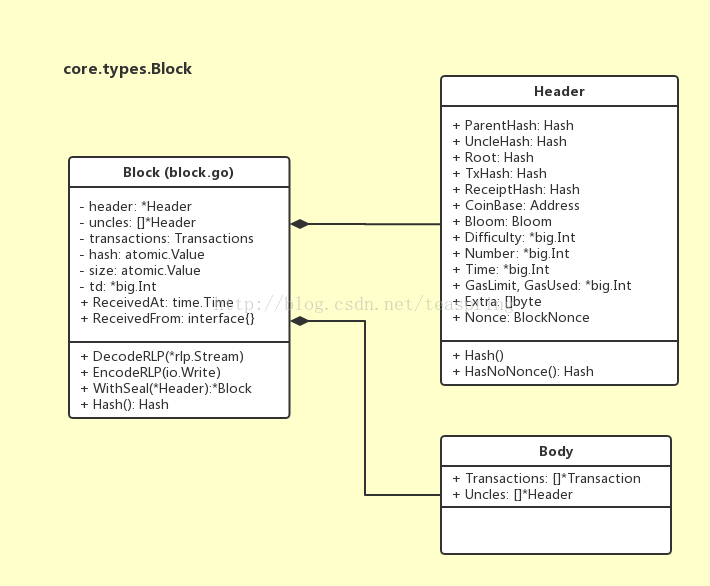
\includegraphics[scale=0.5]{block.png}
	\caption{Block}
	\label{block}
\end{figure}

\Emph{Header部分}

Header是Block的核心,注意到它的成员变量全都是公共的,这使得它可以很方便的向调用者提供关于Block属性的操作。Header的成员变量全都很重要,值得细细理解:

\begin{itemize}

\item \Emph{ParentHash}:指向父区块(parentBlock)的指针。除了创世块(Genesis Block)外,每个区块有且只有一个父区块。

\item \Emph{Coinbase}:挖掘出这个区块的作者地址。在每次执行交易时系统会给与一定补偿的Ether,这笔金额就是发给这个地址的。

\item \Emph{UncleHash}:Block结构体的成员uncles的RLP哈希值。uncles是一个Header数组,它的存在,颇具匠心。

\item \Emph{Root}:StateDB中的“state Trie”的根节点的RLP哈希值。Block中,每个账户以stateObject对象表示,账户以Address为唯一标示,其信息在相关交易(Transaction)的执行中被修改。所有账户对象可以逐个插入一个Merkle-PatricaTrie(MPT)结构里,形成“state Trie”。

\item \Emph{TxHash}: Block中 “tx Trie”的根节点的RLP哈希值。Block的成员变量transactions中所有的tx对象,被逐个插入一个MPT结构,形成“tx Trie”。

\item \Emph{ReceiptHash}:Block中的 "Receipt Trie”的根节点的RLP哈希值。Block的所有Transaction执行完后会生成一个Receipt数组,这个数组中的所有Receipt被逐个插入一个MPT结构中,形成"Receipt Trie"。

\item \Emph{Bloom}:Bloom过滤器(Filter),用来快速判断一个参数Log对象是否存在于一组已知的Log集合中。

\item \Emph{Difficulty}:区块的难度。Block的Difficulty由共识算法基于parentBlock的Time和Difficulty计算得出,它会应用在区块的‘挖掘’阶段。

\item \Emph{Number}:区块的序号。Block的Number等于其父区块Number +1。

\item \Emph{Time}:区块“应该”被创建的时间。由共识算法确定,一般来说,要么等于parentBlock.Time + 10s,要么等于当前系统时间。

\item \Emph{GasLimit}:区块内所有Gas消耗的理论上限。该数值在区块创建时设置,与父区块有关。具体来说,根据父区块的GasUsed同GasLimit * 2/3的大小关系来计算得出。

\item \Emph{GasUsed}:区块内所有Transaction执行时所实际消耗的Gas总和。

\item \Emph{Nonce}:一个64bit的哈希数,它被应用在区块的"挖掘"阶段,并且在使用中会被修改。
\end{itemize}

Merkle-PatriciaTrie(MPT)是Ethereum用来存储区块数据的核心数据结构。最简单理解是一个倒置的树形结构,每个节点可能有若干个子节点,关于MPT在Ethereum中的实现细节在下文有专门介绍。

Root,TxHash和ReceiptHash,分别取自三个MPT类型对象:stateTrie, txTrie, 和receiptTrie的根节点哈希值。用一个32byte的哈希值,来代表一个有若干节点的树形结构(或若干元素的数组),这是为了加密。比如在Block的同步过程中,通过比对收到的TxHash,可以确认数组成员transactions是否同步完整。

三者当中,TxHash和ReceiptHash的生成稍微特殊一点,因为这两的数据来源是数组,而不像stateTrie原本就存在。如何将数组转化成MPT结构?考虑到MPT专门存储[k,v]类型数据,代码里利用了点小技巧:将数组中每个元素的索引作为k,该元素的RLP编码值作为v,组成一个[k,v]键值对作为一个节点,这样所有数组元素作为节点逐个插入一个初始化为空的MPT,形成MPT结构。

在stateTrie,txTrie,receiptTrie这三个MPT结构的产生时间上,receiptTrie 必须在Block的所有交易执行完成才能生成;txTrie 理论上只需tx数组transactions即可,不过依然被限制在所有交易执行完后才生成;最有趣的是stateTrie,由于它存储了所有账户的信息,比如余额,发起交易次数,虚拟机指令数组等等,所以随着每次交易的执行,stateTrie 其实一直在变化,这就使得Root值也在变化中。于是StateDB 定义了一个函数IntermediateRoot(),用来生成那一时刻的Root值:

\begin{lstlisting}

// /core/types/block.go

// Block represents an entire block in the Ethereum blockchain.
type Block struct {
  header       *Header
  uncles       []*Header
  transactions Transactions

  // caches
  hash atomic.Value
  size atomic.Value

  // Td is used by package core to store the total difficulty
  // of the chain up to and including the block.
  td *big.Int

  // These fields are used by package eth to track
  // inter-peer block relay.
  ReceivedAt   time.Time
  ReceivedFrom interface{}
}

//go:generate gencodec -type Header -field-override headerMarshaling -out gen\_header\_json.go

// Header represents a block header in the Ethereum blockchain.
type Header struct {
  ParentHash  common.Hash    `json:"parentHash"       gencodec:"required"`
  UncleHash   common.Hash    `json:"sha3Uncles"       gencodec:"required"`
  Coinbase    common.Address `json:"miner"            gencodec:"required"`
  Root        common.Hash    `json:"stateRoot"        gencodec:"required"`
  TxHash      common.Hash    `json:"transactionsRoot" gencodec:"required"`
  ReceiptHash common.Hash    `json:"receiptsRoot"     gencodec:"required"`
  Bloom       Bloom          `json:"logsBloom"        gencodec:"required"`
  Difficulty  *big.Int       `json:"difficulty"       gencodec:"required"`
  Number      *big.Int       `json:"number"           gencodec:"required"`
  GasLimit    uint64         `json:"gasLimit"         gencodec:"required"`
  GasUsed     uint64         `json:"gasUsed"          gencodec:"required"`
  Time        *big.Int       `json:"timestamp"        gencodec:"required"`
  Extra       []byte         `json:"extraData"        gencodec:"required"`
  MixDigest   common.Hash    `json:"mixHash"          gencodec:"required"`
  Nonce       BlockNonce     `json:"nonce"            gencodec:"required"`
}

\end{lstlisting}

详细解释:https://blog.csdn.net/teaspring/article/details/75390210 Header部分
区块是交易的集合

\begin{lstlisting}

// core/state/statedb.go
func (s *StateDB) IntermediateRoot(deleteEmptyObjects bool) common.Hash

\end{lstlisting}

这个函数的返回值,代表了所有账户信息的一个即时状态。

关于Header.Root的生成时间,在上篇帖子提到的交易执行过程中,交易执行的入口函数StateProcessor.Process()在返回前调用了Engine.Finalize()。正是这个Finalize(),在内部调用上述IntermediateRoot()函数并赋值给header.Root。所以Root值就是在该区块所有交易完成后,所有账户信息的即时状态。

\Emph{Body结构体}

Block的成员变量td 表示的是整个区块链表从源头创世块开始,到当前区块截止,累积的所有区块Difficulty之和,td 取名totalDifficulty。从概念上可知,某个区块与父区块的td之差,就等于该区块Header带有的Difficulty值。

Body可以理解为Block里的数组成员集合,它相对于Header需要更多的内存空间,所以在数据传输和验证时,往往与Header是分开进行的。

Uncles是Body非常特别的一个成员,从业务功能上说,它并不是Block结构体必须的,它的出现当然会占用整个Block计算哈希值时更长的时间,目的是为了抵消整个Ethereum网络中那些计算能力特别强大的节点会对区块的产生有过大的影响力,防止这些节点破坏“去中心化”这个根本宗旨。官方描述可见ethereum-wiki

\Emph{Block的唯一标识符}

同Ethereum世界里的其他对象类似,Block对象的唯一标识符,就是它的(RLP)哈希值。需要注意的是,Block的哈希值,等于其Header成员的(RLP)哈希值。

\begin{lstlisting}


// core/types/Block.go
func (b *Block) Hash() common.Hash {
    if hash := b.hash.Load(); hash != nil {
        return hash.(common.Hash)
    }
    v := b.header.Hash()
    b.hash.Store(v)
    return v
}
func (h *Header) Hash() common.Hash {
    return rlpHash(h)
}


\end{lstlisting}

小技巧:Block的成员hash会缓存上一次Header计算出的哈希值,以避免不必要的计算。
Block的哈希值等于其Header的(RLP)哈希值,这就从根本上明确了Block(结构体)和Header表示的是同一个区块对象。考虑到这两种结构体所占内存空间的差异,这种设计可以带来很多便利。比如在数据传输时,完全可以先传输Header对象,验证通过后再传输Block对象,收到后还可以利用二者的成员哈希值做相互验证。

\Emph{成员分散存储在底层数据库}

Header和Block的主要成员变量,最终还是要存储在底层数据库中。Ethereum 选用的是LevelDB, 属于非关系型数据库,存储单元是[k,v]键值对。我们来看看具体的存储方式(core/database\_util.go)

\begin{tabular}{|l|l|}

\hline
\Emph{key} & \Emph{value} \\
\hline
'h' + num + hash	&	header's RLP raw data \\
\hline
'h' + num + hash + 't'	&	td \\
\hline
'h' + num + 'n'		&	hash \\
\hline
'H' + hash	&	num \\
\hline
'b' + num + hash	&	body's RLP raw data \\
\hline
'r' + num + hash	&	receipts RLP \\
\hline
'l' + hash	&	tx/receipt lookup metadata \\
\hline

\end{tabular}

这里的hash就是该Block(或Header)对象的RLP哈希值,在代码中也被称为canonical hash;num是Number的uint64类型,大端(big endian)整型数。可以发现,num 和 hash是key中出现最多的成分;同时num和hash还分别作为value被单独存储,而每当此时则另一方必组成key。这些信息都在强烈的暗示,num(Number)和hash是Block最为重要的两个属性:num用来确定Block在整个区块链中所处的位置,hash用来辨识惟一的Block/Header对象。

通过以上的设计,Block结构体的所有重要成员,都被存储进了底层数据库。当所有Block对象的信息都已经写进数据库后,我们就可以使用BlockChain结构体来处理整个块链。

\subsection{HeaderChain和BlockChain}

BlockChain结构体被用来管理整个区块单向链表,在一个Ethereum客户端软件(比如钱包)中,只会有一个BlockChain对象存在。同Block/Header的关系类似,BlockChain还有一个成员变量类型是HeaderChain, 用来管理所有Header组成的单向链表。当然,HeaderChain在全局范围内也仅有一个对象,并被BlockChain持有(准确说是HeaderChain只会被BlockChain和LightChain持有,LightChain类似于BlockChain,但默认只处理Headers,不过依然可以下载bodies和receipts)。它们的UML关系图如下所示:

\begin{figure}
	\centering
	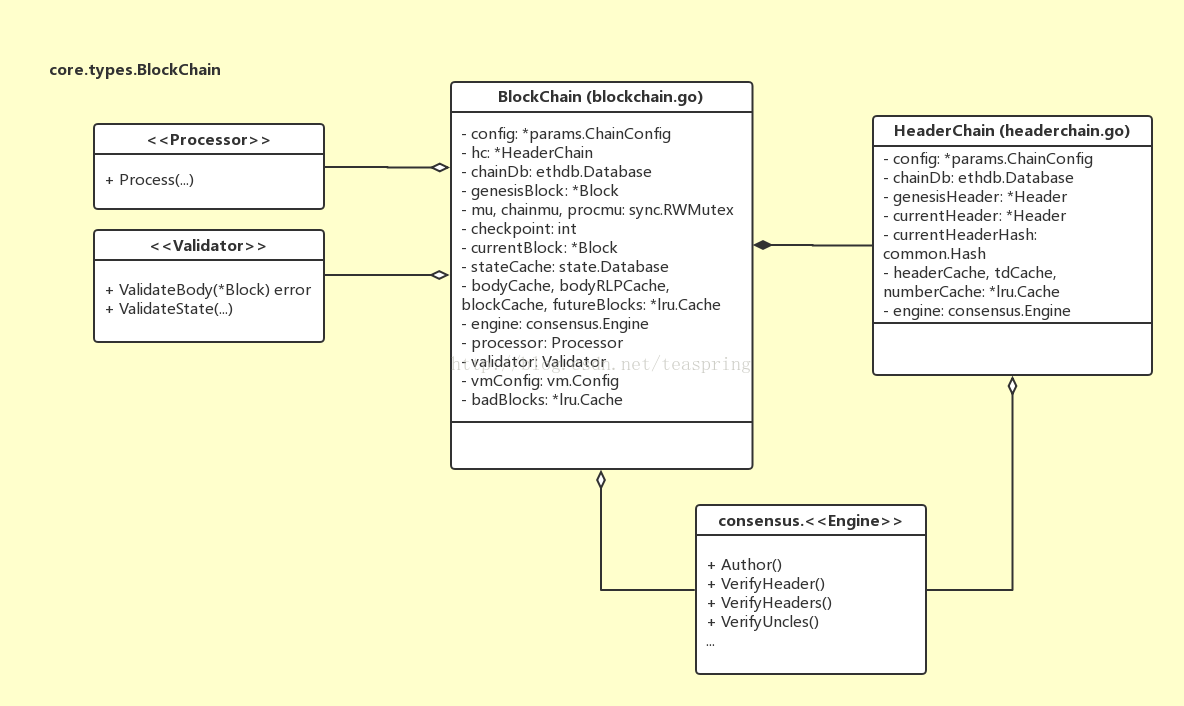
\includegraphics[scale=0.4]{blockchain.png}
	\caption{BlockChain}
	\label{blockchain}
\end{figure}

在结构体的设计上,BlockChain 同HeadeChain有诸多类似之处。比如二者都有相同的ChainConfig对象,有相同的Database接口行为变量以提供[k,v]数据的读取和写入;BlockChain 有成员genesisBlock和currentBlock,分别对应创世块和当前块,而HeaderChain则有genesisHeader和currentHeader;BlockChain 有bodyCache,blockCache 等成员用以缓存高频调用对象,而HeaderChain则有headerCache, tdCache, numberCache等缓存成员变量。除此之外,BlockChain 相对于HeaderChain主要增多了Processor和Validator两个接口行为变量,前者用以执行所有交易对象,后者可以验证诸如Body等数据成员的有效性。

Engine是共识算法定义的行为接口。共识算法是整个数字货币体系最重要的概念之一,它在理论上的完整性,有力的支撑了“去中心化”这个伟大设想的实现。落实在代码层面,consensus.Engine就是Ethereum系统里共识算法的一个主要行为接口,它基于符合某种共识算法规范的算法库,提供包括VerifyHeaders(),VerifyUncles()等一系列涉及到数据合法性的关键函数。不仅仅BlockChain和HeaderChain结构体,在Ethereum系统里,所有跟验证区块对象相关的操作都会调用Engine行为接口来完成。目前存在两种共识算法规范,一种是基于运算能力(proof-of-work),叫Ethash;另一种基于某个投票机制(proof-of-authority),叫Clique。具体内容在之后的文章中会有更多展开。

\Emph{区块链的操作}

从逻辑上讲,既然BlockChain和HeaderChain都管理着一个类似单向链表的结构,那么它们提供的操作方法肯定包括插入,删除,和查找。

查找比较简单,以BlockChain为例,它有一个成员currentBlock,指向当前最新的Block,而HeaderChain也有一个类似的成员currentHeader。除此之外,底层数据库里还分别存有当前最新Block和Header的canonical hash:
\begin{center}

\begin{tabular}{|l|l|}

\hline
\Emph{key} & \Emph{value} \\
\hline
"LastHeader"	&	hash \\
\hline
"LastBlock"	&	hash \\
\hline
"LastFast"	&	hash \\
\hline
\end{tabular}

\end{center}

这里“LastFast”所存储的是在一种特别的同步方式FastSync下,最新Block的canonical hash。FastSync相比于FullSync,可以仅仅同步Header而不考虑Body,故此得名Fast。
以BlockChain为例,通过"LastBlock"为key从数据库中获取最新的Block之后,用num逐一遍历,得到目标Block的num后,用'h'+num+'n'作key,就可以从数据库中获取目标canonical hash。

插入和删除。区块链跟普通单向链表有一点非常明显的不同,在于Header的前向指针ParentHash是不能修改的,即当前区块的父区块是不能修改的。所以在插入的实现中,当决定写入一个新的Header进底层数据库时,从这个Header开始回溯,要保证它的parent,以及parent的parent等等,都已经写入数据库了。只有这样,才能确保从创世块(num为0)起始,直到当前新写入的区块,整个链式结构是完整的,没有中断或分叉。删除的情形也类似,要从num最大的区块开始,逐步回溯。在BlockChain的操作里,删除一般是伴随着插入出现的,即当需要插入新区块时,才可能有旧的区块需要被删除,这种情形在代码里被称为reorg。

\subsection{精巧的Merkle-PatriciaTrie}

Ethereum 使用的Merkle-PatriciaTrie(MPT)结构,源自于Trie结构,又分别继承了PatriciaTrie和MerkleTree的优点,并基于内部数据的特性,设计了全新的节点体系和插入/载入机制。

Trie,又称为字典树或者前缀树(prefix tree),属于查找树的一种。它与平衡二叉树的主要不同点包括:每个节点数据所携带的key不会存储在Trie的节点中,而是通过该节点在整个树形结构里位置来体现;同一个父节点的子节点,共享该父节点的key作为它们各自key的前缀,因此根节点key为空;待存储的数据只存于叶子节点中,非叶子节点帮助形成叶子节点key的前缀。下图来自wiki-Trie,展示了一个简单的Trie结构。

\begin{figure}
	\centering
	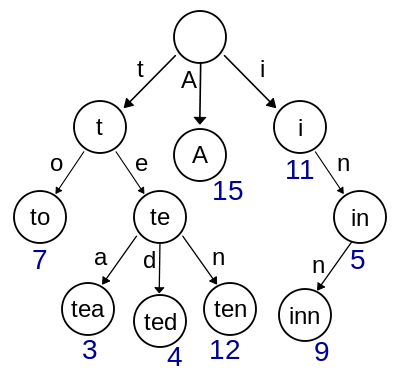
\includegraphics[scale=0.5]{trie.png}
	\caption{Trie}
	\label{trie}
\end{figure}

\Emph{PatriciaTrie},又被称为RadixTree或紧凑前缀树(compact prefix tree),是一种空间使用率经过优化的Trie。与Trie不同的是,PatriciaTrie里如果存在一个父节点只有一个子节点,那么这个父节点将与其子节点合并。这样可以缩短Trie中不必要的深度,大大加快搜索节点速度。

\Emph{MerkleTree},也叫哈希树(hash tree),是密码学的一个概念,注意理论上它不一定是Trie。在哈希树中,叶子节点的标签是它所关联数据块的哈希值,而非叶子节点的标签是它的所有子节点的标签拼接而成字符串的哈希值。哈希树的优势在于,它能够对大量的数据内容迅速作出高效且安全的验证。假设一个hash tree中有n个叶子节点,如果想要验证其中一个叶子节点是否正确-即该节点数据属于源数据集合并且数据本身完整,所需哈希计算的时间复杂度是是O(log(n)),相比之下hash list大约需要时间复杂度O(n)的哈希计算,hash tree的表现无疑是优秀的。

\begin{figure}
	\centering
	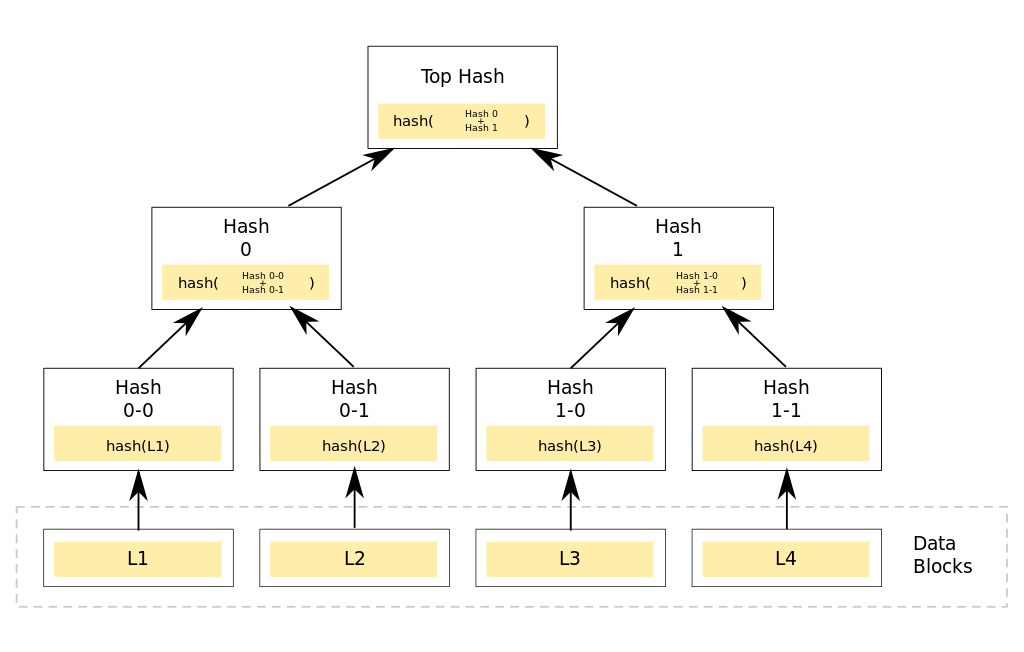
\includegraphics[scale=0.45]{merkletree.png}
	\caption{MerkleTree}
	\label{merkleTree}
\end{figure}

上图来自wiki-MerkleTree,展示了一个简单的二叉哈希树。四个有效数据块L1-L4,分别被关联到一个叶子节点上。Hash0-0和Hash0-1分别等于数据块L1和L2的哈希值,而Hash0则等于Hash0-0和Hash0-1二者拼接成的新字符串的哈希值,依次类推,根节点的标签topHash等于Hash0和Hash1二者拼接成的新字符串的哈希值。

哈希树最主要的应用场景是p2p网络中的数据传输。因为p2p网络中可能存在未知数目的不可信数据源,所以确保下载到的数据正确可信并且无损坏无改动,就显得非常重要。哈希树可用来解决这个问题:每个待下载文件按照某种方式分割成若干小块后,组成类似上图的哈希树。首先从一个绝对可信的数据源获取该文件对应哈希树的根节点哈希值(top hash),有了这个可靠的top hash后,就可以开始从整个p2p网络下载文件。不同的数据部分可以从不同的源下载,由于哈希树中任意的分支树都可以单独验证哈希值,所以一旦发现任何数据部分无法通过验证,都可以切换到其他数据源进行下载那部分数据。最终,完整下载文件所对应哈希树的top hash值,一定要与我们的可靠top hash相等。

\Emph{Merkle-Patricia Trie(MPT)的实现}

MPT是Ethereum自定义的Trie型数据结构。在代码中,trie.Trie结构体用来管理一个MPT结构,其中每个节点都是行为接口Node的实现类。下图是Trie结构体和node接口族的UML关系图:

\begin{figure}
	\centering
	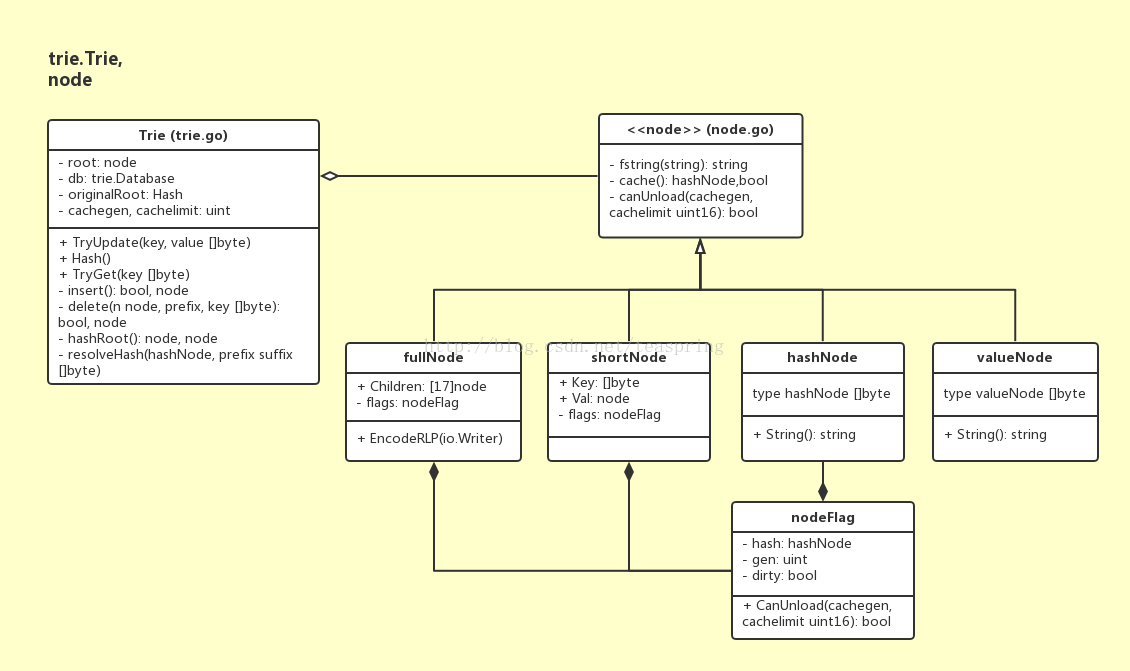
\includegraphics[scale=0.4]{mpt.png}
	\caption{Merkle-Patricia Trie}
	\label{mpt}
\end{figure}

在Trie结构体中,成员root始终作为整个MPT的根节点;originalRoot的作用是在创建Trie对象时承接入参hashNode;cacheGen是cache次数的计数器,每次Trie的变动提交后(写入的对象可由外部参数传入),cacheGen自增1。Trie结构体提供包括对节点的插入、删除、更新,所有节点改动的提交(写入到传入参数),以及返回整个MPT的哈希值。

node接口族担当整个MPT中的各种节点,node接口分四种实现: fullNode,shortNode,valueNode,hashNode,其中只有fullNode和shortNode可以带有子节点。

\Emph{fullNode} 是一个可以携带多个子节点的父(枝)节点。它有一个容量为17的node数组成员变量Children,数组中前16个空位分别对应16进制(hex)下的0-9a-f,这样对于每个子节点,根据其key值16进制形式下的第一位的值,就可挂载到Children数组的某个位置,fullNode本身不再需要额外key变量;Children数组的第17位,留给该fullNode的数据部分。fullNode明显继承了原生trie的特点,而每个父节点最多拥有16个分支也包含了基于总体效率的考量。

\Emph{shortNode} 是一个仅有一个子节点的父(枝)节点。它的成员变量Val指向一个子节点,而成员Key是一个任意长度的字符串(字节数组[]byte)。显然shortNode的设计体现了PatriciaTrie的特点,通过合并只有一个子节点的父节点和其子节点来缩短trie的深度,结果就是有些节点会有长度更长的key。

\Emph{valueNode} 充当MPT的叶子节点。它其实是字节数组[]byte的一个别名,不带子节点。在使用中,valueNode就是所携带数据部分的RLP哈希值,长度32byte,数据的RLP编码值作为valueNode的匹配项存储在数据库里。

这三种类型覆盖了一个普通Trie(也许是PatriciaTrie)的所有节点需求。任何一个[k,v]类型数据被插入一个MPT时,会以k字符串为路径沿着root向下延伸,在此次插入结束时首先成为一个valueNode,k会以自顶点root起到到该节点止的key path形式存在。但之后随着其他节点的不断插入和删除,根据MPT结构的要求,原有节点可能会变化成其他node实现类型,同时MPT中也会不断裂变或者合并出新的(父)节点。比如:

\begin{itemize}

\item 假设一个shortNode S已经有一个子节点A,现在要新插入一个子节点B,那么会有两种可能,要么新节点B沿着A的路径继续向下,这样S的子节点会被更新;要么S的Key分裂成两段,前一段分配给S作为新的Key,同时裂变出一个新的fullNode作为S的子节点,以同时容纳B,以及需要更新的A。

\item 如果一个fullNode原本只有两个子节点,现在要删除其中一个子节点,那么这个fullNode就会退化为shortNode,同时保留的子节点如果是shortNode,还可以跟它再合并。

\item 如果一个shortNode的子节点是叶子节点同时又被删除了,那么这个shortNode就会退化成一个valueNode,成为一个叶子节点。

\end{itemize}

诸如此类的情形还有很多,提前设想过这些案例,才能正确实现MPT的插入/删除/查找等操作。当然,所有查找树(search tree)结构的操作,免不了用到递归。

\Emph{特殊的那个 - hashNode}

hashNode 跟valueNode一样,也是字符数组[]byte的一个别名,同样存放32byte的哈希值,也没有子节点。不同的是,hashNode是fullNode或者shortNode对象的RLP哈希值,所以它跟valueNode在使用上有着莫大的不同。

在MPT中,hashNode几乎不会单独存在(有时遍历遇到一个hashNode往往因为原本的node被折叠了),而是以nodeFlag结构体的成员(nodeFlag.hash)的形式,被fullNode和shortNode间接持有。一旦fullNode或shortNode的成员变量(包括子结构)发生任何变化,它们的hashNode就一定需要更新。所以在trie.Trie结构体的insert(),delete()等函数实现中,可以看到除了新创建的fullNode、shortNode,那些子结构有所改变的fullNode、shortNode的nodeFlag成员也会被重设,hashNode会被清空。在下次trie.Hash()调用时,整个MPT自底向上的遍历过程中,所有清空的hashNode会被重新赋值。这样trie.Hash()结束后,我们可以得到一个根节点root的hashNode,它就是此时此刻这个MPT结构的哈希值。上文中提到的,Block的成员变量Root、TxHash、ReceiptHash的生成,正是源出于此。

明显的,hashNode体现了MerkleTree的特点:每个父节点的哈希值来源于所有子节点哈希值的组合,一个顶点的哈希值能够代表一整个树形结构。valueNode加上之前的fullNode,shortNode,valueNode,构成了一个完整的Merkle-PatriciaTrie结构,很好的融合了各种原型结构的优点,又根据Ethereum系统的实际情况,作了实际的优化和平衡。MPT这个数据结构在设计中的种种细节,的确值得好好品味。

\Emph{函数实现}

代码方面,创建新nodeFlag对象的函数叫newFlags()。在nodeFlag初始化过程中,bool成员dirty置为true,表明了所代表的父节点有改动需要提交,同时hashNode成员hash,直接设空。

\begin{lstlisting}

// trie/trie.go
func (t *Trie) newFlag() nodeFlag {
    return nodeFlag{dirty: true, gen: t.cacheGen}
}

\end{lstlisting}


每个hashNode被赋值的过程,就是它所代表的fullNode或shortNode被折叠(collapse)的过程。基于效率和数据安全考虑,trie.Trie仅提供整个MPT结构的折叠操作Hash()函数,它默认从顶点root开始遍历。

\begin{lstlisting}


func (t *Trie) Hash() common.Hash {
    hash, cached, _ := t.hashRoot(db:nil)
    t.root = hash
    return ...
}
func (t *Trie) hashRoot(db DatabaseWriter) (node, node, error) {
    if (t.root == nil) {...}
    h := newHasher(t.cachegen, t.cachelimit)
    return h.hash(t.root, db, force:true)
}

\end{lstlisting}

hashRoot()函数内部调用Hasher结构体进行折叠操作:

\begin{lstlisting}

// trie/hasher.go
func (h *hasher) hash(n node, db DatabaseWriter, force bool) (hash node, cached node, error)
func (h *hasher) hashChildren(original node, db DatabaseWriter) (hash node, cached node, error)
func (h *hasher) store(n node, db DatabaseWriter, force bool) (node, error)

\end{lstlisting}

折叠node的入口是hasher.hash(),在执行中,hash()和hashChiildren()相互调用以遍历整个MPT结构,store()对节点作RLP哈希计算。折叠node的基本逻辑是:如果node没有子节点,那么直接返回;如果这个node带有子节点,那么首先将子节点折叠成hashNode。当这个node的子节点全都变成哈希值hashNode之后,再对这个node作RLP+哈希计算,得到它的哈希值,亦即hashNode。
注意到hash()和hashChildren()返回两个node类型对象,第一个@hash是入参n经过折叠的hashNode哈希值,第二个@cached是没有经过折叠的n,并且n的hashNode还被赋值了。
由于Hasher.hash()有一个数据库接口类型的参数,这样在折叠MPT过程中,如果db不为空,就把每次计算hashNode时的哈希值和它对应的节点RLP编码值一起存进数据库里,这也正是Commit()的逻辑。

\begin{lstlisting}
func (t *Trie) Commit() (root hash, error) {
    if t.db == nil {...}
    return t.CommitTo(t.db)
}
func (t *Trie) CommitTo(db DatabaseWriter) (root common.Hash, error) {
    hash, cached, error := t.hashRoot(db)
    t.root = cached
    ...
}

\end{lstlisting}

回看一下Trie.Hash(),它在调用hashRoot()时,传入的是空值db。只有显式调用Commit()或者CommitTo()才可以提交数据,所以Hash()多次调用也是安全的。
在MPT的查找,插入,删除中,如果遍历过程中遇到一个hashNode,首先需要从数据库里以这个哈希值为k,读取出相匹配的v,然后再将v解码恢复成fullNode或shortNode。在代码中这个过程叫resolve。

\begin{lstlisting}

// trie/trie.go
func (t *trie) resolve(n, prefix) (node,error) {
    if n, ok := n.(hashNode); ok {
        return resolveHash(n, prefix)
    }
    return n, nil
}
func (t *Trie) resolveHash(n hashNode, prefix []byte) (node,error) {
    enc, err := t.db.Get(n)
    ...
    dec := mustDecodeNode(n, enc, t.cachegen)
    return dec, nil
}

\end{lstlisting}

这样,涉及到hashNode的所有操作就基本完整了。

\Emph{MPT中对key的编码}

当[k,v]数据插入MPT时,它们的k(key)都必须经过编码。这时对key的编码,要保证原本是[]byte类型的key能够以16进制形式按位进入fullNode.Children[],因为Children[]数组最多只能容纳16个子节点。相应的,Ethereum代码中在这里定义了一种编码方式叫Hex,将1byte的字符大小限制在4bit(16进制)以内。

先来看Hex编码的实现,这里将原本[]byte形式称之为keybytes,Hex编码的基本逻辑如下图:

\begin{figure}
	\centering
	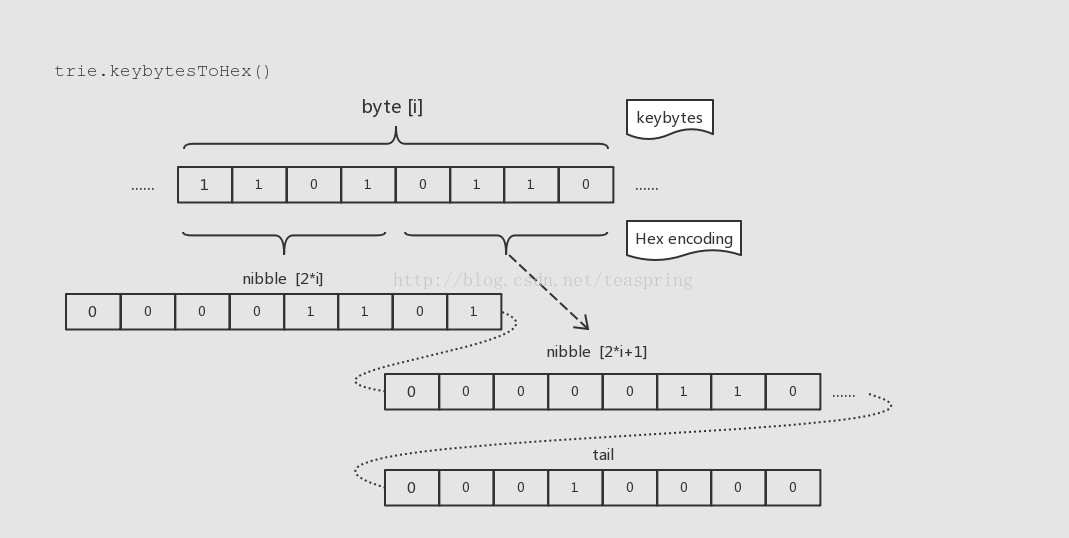
\includegraphics[scale=0.45]{keybytes.png}
	\caption{keybytes}
	\label{keybytes}
\end{figure}

很简单,就是将keybytes中的1byte信息,将高4bit和低4bit分别放到两个byte里,最后在尾部加1byte标记当前属于Hex格式。这样新产生的key虽然形式还是[]byte,但是每个byte大小已经被限制在4bit以内,代码中把这种新数据的每一位称为nibble。这样经过编码之后,带有[]nibble格式的key的数据就可以顺利的进入fullNode.Children[]数组了。

Hex编码虽然解决了key是keybytes形式的数据插入MPT的问题,但代价也很大,就是数据冗余。典型的如shortNode,目前Hex格式下的Key,长度会变成是原来keybytes格式下的两倍。这一点对于节点的哈希计算,比如计算hashNode,影响很大。所以Ethereum又定义了另一种编码格式叫Compact,用来对Hex格式进行优化。

Compact编码又叫hex prefix编码,它的主要意图是将Hex格式的字符串恢复到keybytes的格式,同时要加入当前Compact格式的标记位,还要考虑在奇偶不同长度Hex格式字符串下,避免引入多余的byte。

\begin{figure}
	\centering
	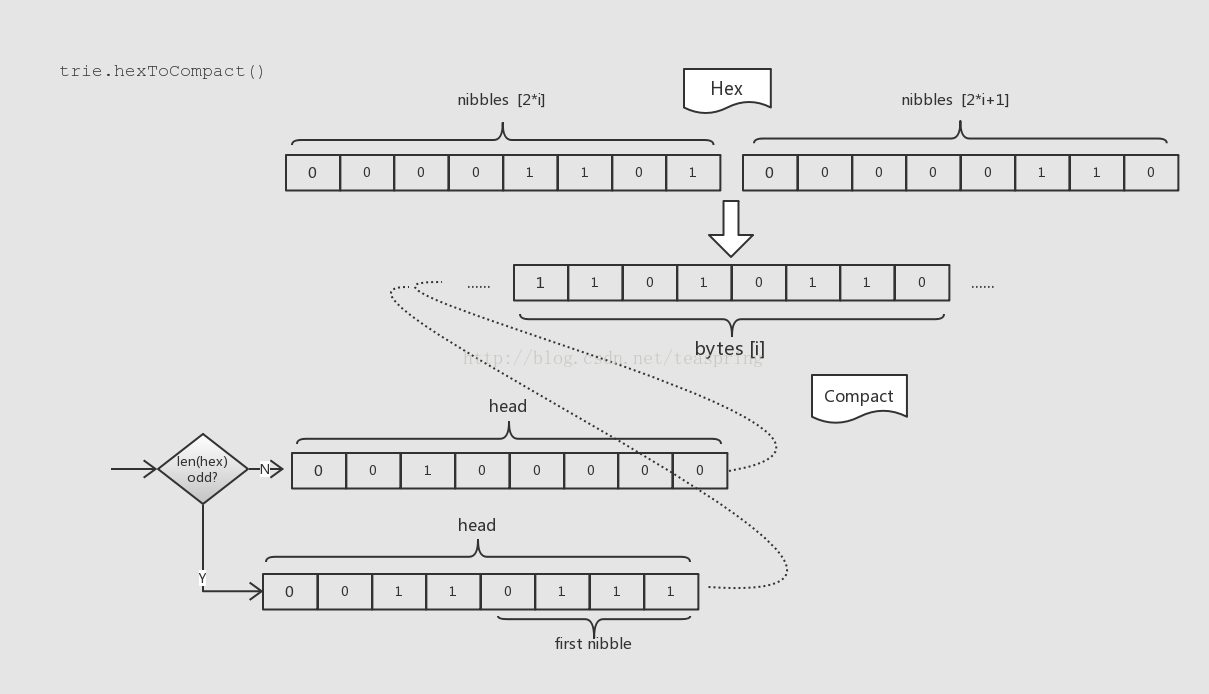
\includegraphics[scale=0.35]{keybytes2.png}
	\caption{keybytes}
	\label{keybytes2}
\end{figure}

如上图所示,Compact编码首先将Hex尾部标记byte去掉,然后将原本每2 nibble的数据合并到1byte;增添1byte在输出数据头部以放置Compact格式标记位;如果输入Hex格式字符串有效长度为奇数,还可以将Hex字符串的第一个nibble放置在标记位byte里的低4bit。

Key编码的设计细节,也体现出MPT整个数据结构设计的思路很完整。

\subsection{数据库体系}

到目前为止,Ethereum系统中区块数据的呈现,组织管理已经介绍了不少,我们可以开始探讨存储部分了。先来看看数据存储部分的UML关系图。

\begin{figure}
	\centering
	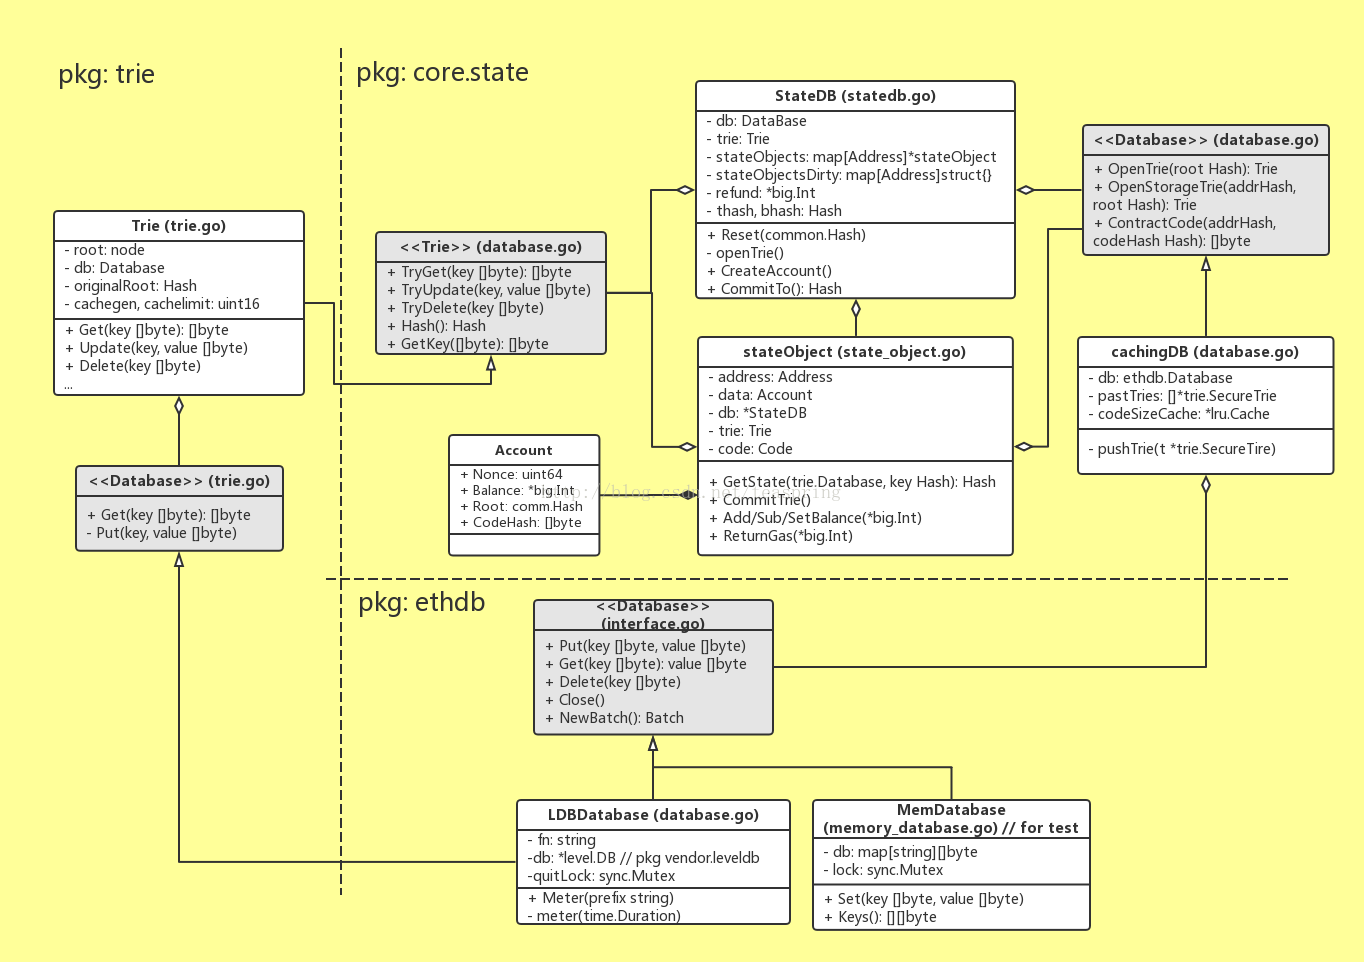
\includegraphics[scale=0.3]{store.png}
	\caption{数据库存储部分关系图}
	\label{store}
\end{figure}

属于Ethereum代码范围内的最底层数据库是ethdb.LDBDatabase,它通过持有一个levelDB的对象,最终为Ethereum世界里所有需要存储/读取[k,b]的需求提供服务。

留意到图中多次出现一种类似的设计模式,比如trie.Trie持有一个本地接口trie.<<Database>>,而后者的具体实现是ethdb.LDBDatabase。这种设计模式其实是golang的语法带来的。在golang中,一个结构体(类)要实现另一个接口的所有方法,不必在结构体声明时显式继承那个接口,只要完全实现那些方法。这样,当一个结构体想调用另一个包路径下结构体的多个方法时,可以声明一个本地接口,带有几个同想要调用方法完全一样的方法,就可以了,这种方式的优点是不同包之间的代码更充分的解耦合。所以在上图中,这些辅助性的本地接口全都被标为灰色,只需要关注实际调用的实现类就好了。

系统设计中,在底层数据库模块和业务模型之间,往往需要设置本地存储模块,它面向业务模型,可以根据业务需求灵活的设计各种存储格式和单元,同时又连接底层数据库,如果底层数据库(或者第三方API)有变动,可以大大减少对业务模块的影响。在Ethereum世界里,StateDB就担任这个角色,它通过大量的stateObject对象集合,管理所有“账户”信息。

\Emph{面向业务的存储模块 - StateDB}

StateDB有一个trie.Trie类型成员trie,它又被称为storage trie或stte trie,这个MPT结构中存储的都是stateObject对象,每个stateObject对象以其地址(20 bytes)作为插入节点的Key;每次在一个区块的交易开始执行前,trie由一个哈希值(hashNode)恢复出来。另外还有一个map结构,也是存放stateObject,每个stateObject的地址作为map的key。那么问题来了,这些数据结构之间是怎样的关系呢?

\begin{figure}
	\centering
	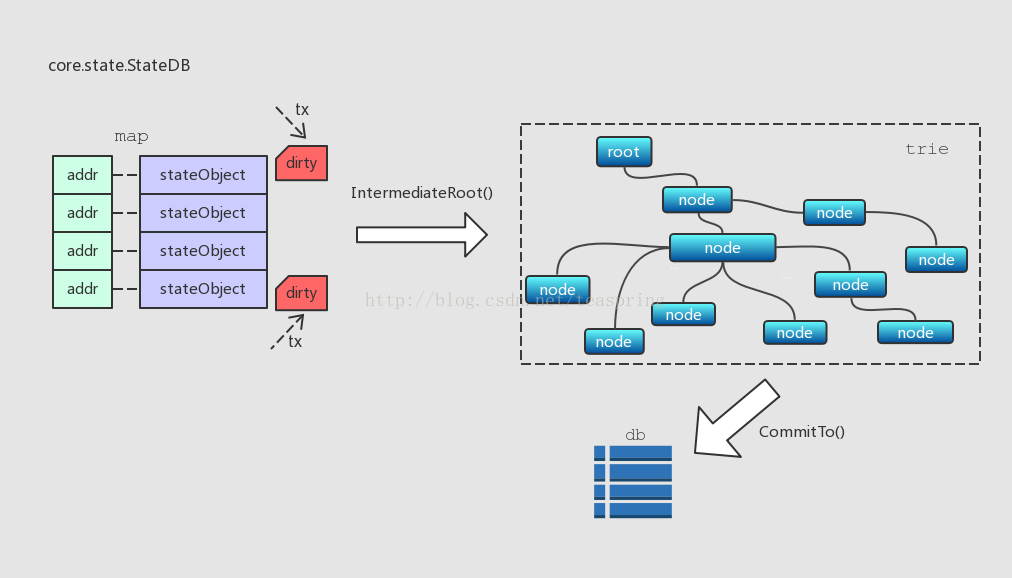
\includegraphics[scale=0.35]{statedb.png}
	\caption{StateDB}
	\label{statedb}
\end{figure}

如上图所示,每当一个stateObject有改动,亦即“账户”信息有变动时,这个stateObject对象会更新,并且这个stateObject会标为dirty,此时所有的数据改动还仅仅存储在map里。当IntermediateRoot()调用时,所有标为dirty的stateObject才会被一起写入trie。而整个trie中的内容只有在CommitTo()调用时被一起提交到底层数据库。可见,这个map被用作本地的一级缓存,trie是二级缓存,底层数据库是第三级,各级数据结构的界限非常清晰,这样逐级缓存数据,每一级数据向上一级提交的时机也根据业务需求做了合理的选择。

\Emph{StateDB中账户状态的版本管理}

StateDB还可以管理账户状态的版本。这个功能用到了几个结构体:journal,revision,先来看看UML关系图:

\begin{figure}
	\centering
	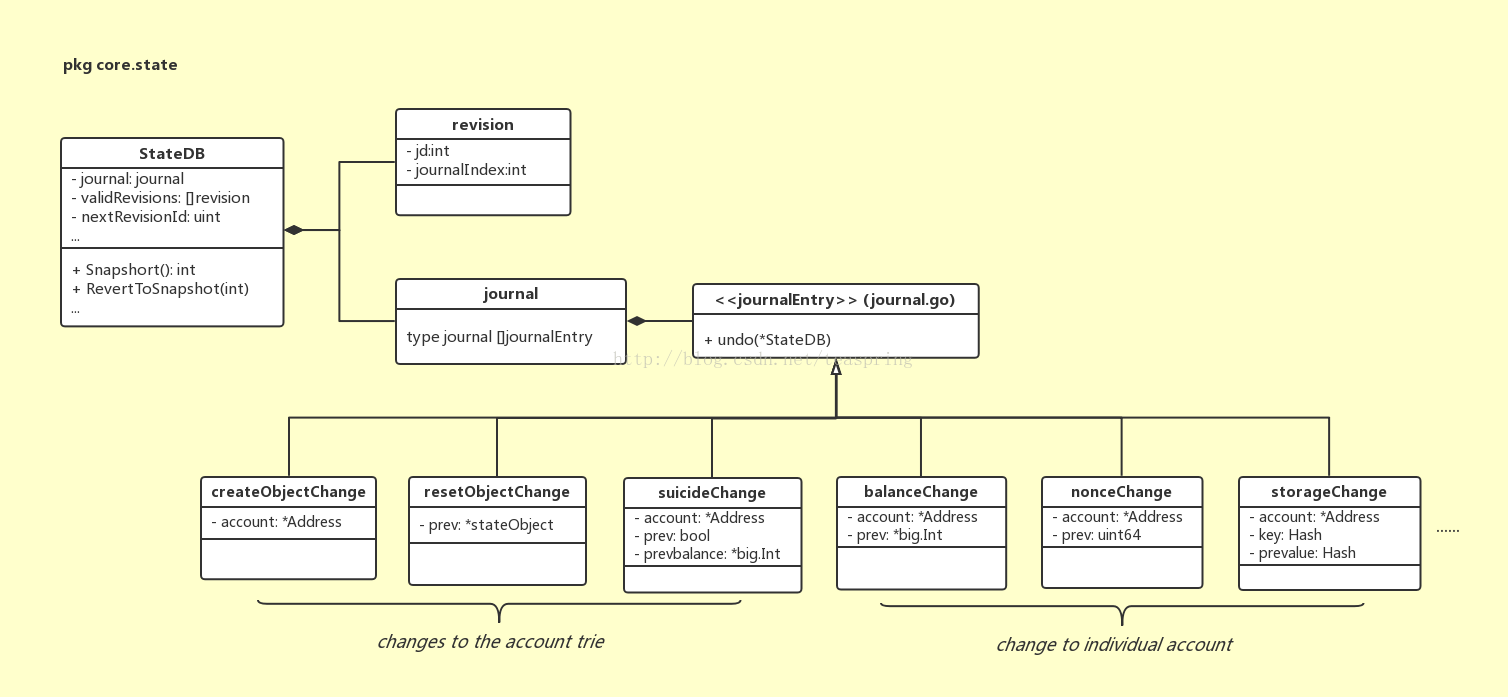
\includegraphics[scale=0.28]{statedb2.png}
	\caption{StateDB中账户状态的版本管理}
	\label{statedb2}
\end{figure}

其中journal对象是journalEntry的散列,长度不固定,可任意添加元素。接口journalEntry存在若干种实现体,描述了从单个账户操作(账户余额,发起合约次数等),到account trie变化(创建新账户对象,账户消亡)等各种最小事件。revision结构体,用来描述一个‘版本’,它的两个整型成员jd和journalIndex,都是基于journal散列进行操作的。

\begin{figure}
	\centering
	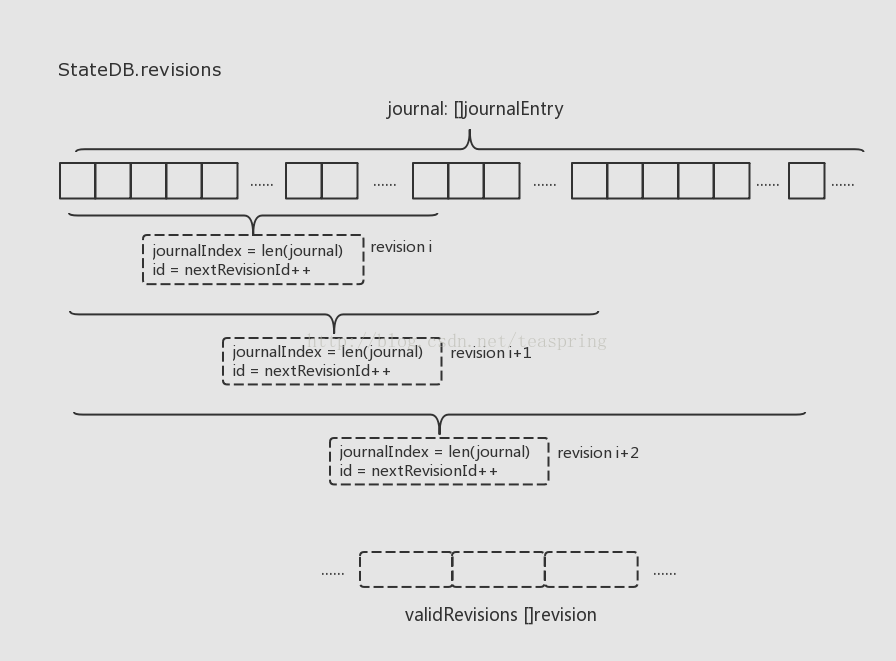
\includegraphics[scale=0.4]{statedb3.png}
	\caption{StateDB.revisions}
	\label{statedb3}
\end{figure}

上图简述了StateDB中账户状态的版本是如何管理的。首先journal散列会随着系统运行不断的增长,记录所有发生过的单位事件;当某个时刻需要产生一个账户状态版本时,代码中相应的是Snapshop()调用,会产生一个新revision对象,记录下当前journal散列的长度,和一个自增1的版本号。

基于以上的设计,当发生回退要求时,只要根据相应的revision中的journalIndex,在journal散列上,根据所记录的所有journalEntry,即可使所有账户回退到那个状态。

\Emph{Ethereum里的账户 - stateObject}

每个stateObject对象管理着Ethereum世界里的一个“账户”。stateObject有一个成员变量data,类型是Accunt结构体,里面存有账户Ether余额,合约发起次数,最新发起合约指令集的哈希值,以及一个MPT结构的顶点哈希值。

stateObject内部也有一个Trie类型的成员trie,被称为storage trie,它里面存放的是一种被称为State的数据。State跟每个账户相关,格式是[Hash, Hash]键值对。有意思的是,stateObject内部也有类似StateDB一样的二级数据缓存机制,用来缓存和更新这些State。

\begin{figure}
	\centering
	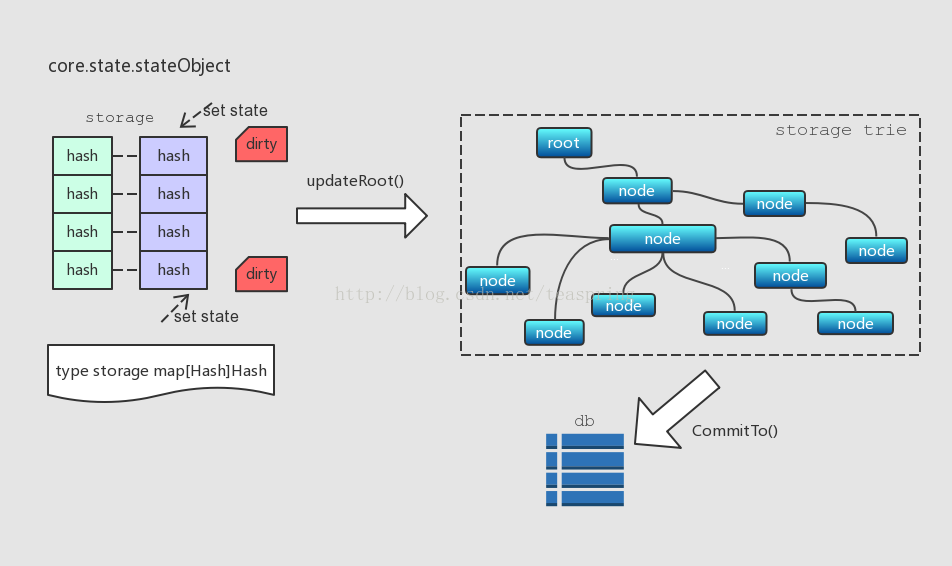
\includegraphics[scale=0.35]{stateObject.png}
	\caption{stateObject}
	\label{stateObject}
\end{figure}

stateObject定义了一种类型名为storage的map结构,用来存放[]Hash,Hash]类型的数据对,也就是State数据。当SetState()调用发生时,storage内部State数据被更新,相应标示为"dirty"。之后,待有需要时(比如updateRoot()调用),那些标为"dirty"的State数据被一起写入storage trie,而storage trie中的所有内容在CommitTo()调用时再一起提交到底层数据库。

State数据略显神秘,目前笔者尚未完全理解它的含义,在代码里,仅仅查到某些合约指令中会调用SetState(),来更新某个stateObject中的State数据。

\Emph{小结}

任何一个系统中,数据部分的占用空间,运行效率当然会影响到整体性能。如何简洁完整的呈现数据,并涵盖业务模型下的大大小小各种需求;如何高效的管理数据,使得插入、删除、查找数据更快速;如何在业务模块和底层数据库之间安排面向业务的、接口友好的本地存储模块,使得内存占用更紧凑,提交和回退数据更加安全等等,都是值得全面思考的。从本文中,可以看到整个Ethereum系统的架构设计、代码实现上,对于以上各个话题都进行了诸多考量,值得同业者学习参考。

\begin{itemize}

\item Block结构体主要分为Header和Body,Header相对轻量,涵盖了Block的所有属性,包括特征标示,前向指针,和内部数据集的验证哈希值等;Body相对重量,持有内部数据集。每个Block的Header部分,Body部分,以及一些特征属性,都以[k,v]形式单独存储在底层数据库中。

\item BlockChain管理Block组成的一个单向链表,HeaderChain管理Header组成的单向链表,并且BlockChain持有HeaderChain。在做插入/删除/查找时,要注意回溯,以及数据库中相应的增删。

\item Merkle-PatriciaTrie(MPT)数据结构用来组织管理[k,v]型数据,它设计了灵活多变的节点体系和编码格式,既融合了多种原型结构的优点,又兼顾了业务需求和运行效率。

\item StateDB作为本地存储模块,它面向业务模型,又连接底层数据库,内部利用两极缓存机制来存储和更新所有代表“账户”的stateObject对象。

\item stateObject除了管理着账户余额等信息之外,也用了类似的两级缓存机制来存储和更新所有的State数据。

\end{itemize}

\section{交易}

\subsection{交易数据结构}

\begin{lstlisting}
/core/types/transaction.go

type Transaction struct {
  data txdata
  // caches
  hash atomic.Value
  sze atomic.Value
  from atomic.Value
}

type txdata struct {
  AccountNonce uint64          `json:"nonce"    gencodec:"required"`
  Price        *big.Int        `json:"gasPrice" gencodec:"required"`
  GasLimit     uint64          `json:"gas"      gencodec:"required"`
  Recipient    *common.Address `json:"to"       rlp:"nil"` // nil means contract creation
  Amount       *big.Int        `json:"value"    gencodec:"required"`
  Payload      []byte          `json:"input"    gencodec:"required"`

  // Signature values
  V *big.Int `json:"v" gencodec:"required"`
  R *big.Int `json:"r" gencodec:"required"`
  S *big.Int `json:"s" gencodec:"required"`

  // This is only used when marshaling to JSON.
  Hash *common.Hash `json:"hash" rlp:"-"`
}

\end{lstlisting}

\paragraph{Price}
Price指的是单位Gas消耗的Ether,它的高低影响着此次tx的交易成本。

\paragraph{GasLimit}
此tx执行过程中所允许消耗消耗资源的总上限,通过这个值,我们可以防止某个tx执行中出现恶意占用资源的问题。

\paragraph{Recipient}
转账转入方地址Recipient可能为空(nil),需要一个地址来完成转账交易。

\paragraph{Payload}
Payload既可以作为所创建合约的指令数组,其中每一个byte作为一个独立的虚拟机指令;也可以作为数据数组,由合约指令进行操作。
合约由EVM创建并执行。

tx的转账转出方地址没有如转入方一样被显示的声明出来,而是被加密隐藏起来了,在以太坊里转入方地址是机密,不能直接暴露。

\subsection{交易数字签名}

\begin{figure}
	\centering
	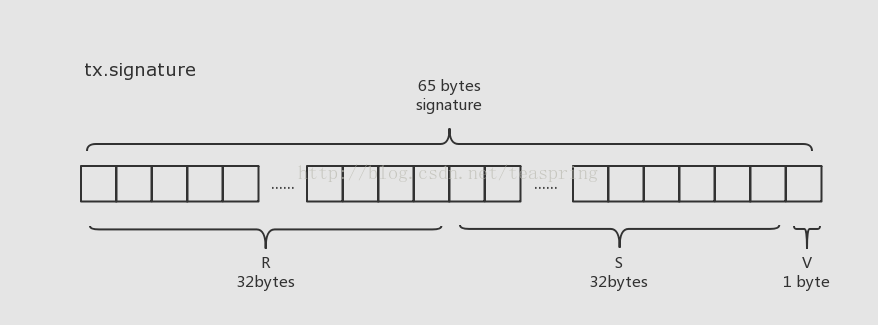
\includegraphics[scale=0.4]{signature.png}
	\caption{Signature}
	\label{signature}
\end{figure}

Ethereum 中每个交易(transaction,tx)对象在被放进block时,都是经过数字签名的,这样可以在后续传输和处理中随时验证tx是否经过篡改。Ethereum 采用的数字签名是椭圆曲线数字签名算法(Elliptic Cure Digital Signature Algorithm,ECDSA)。ECDSA 相比于基于大质数分解的RSA数字签名算法,可以在提供相同安全级别(in bits)的同时,仅需更短的公钥(public key)。关于ECDSA的算法理论和实现细节,本系列会有另外一篇文章专门加以介绍。这里需要特别留意的是,tx的转帐转出方地址,就是对该tx对象作ECDSA签名计算时所用的公钥publicKey。

Ethereum中的数字签名计算过程所生成的签名(signature), 是一个长度为65bytes的字节数组,它被截成三段放进tx中,前32bytes赋值给成员变量R, 再32bytes赋值给S,末1byte赋给V,当然由于R、S、V声明的类型都是*big.Int, 上述赋值存在[]byte -> big.Int的类型转换。

当需要恢复出tx对象的转帐转出方地址时(比如在需要执行该交易时),Ethereum 会先从tx的signature中恢复出公钥,再将公钥转化成一个common.Address类型的地址,signature由tx对象的三个成员变量R,S,V转化成字节数组[]byte后拼接得到。

Ethereum 对此定义了一个接口Signer, 用来执行挂载签名,恢复公钥,对tx对象做哈希等操作。

\begin{lstlisting}
/core/types/transaction_signing.go


// Signer encapsulates transaction signature handling. Note that this interface is not a
// stable API and may change at any time to accommodate new protocol rules.
type Signer interface {
	// Sender returns the sender address of the transaction.
	Sender(tx *Transaction) (common.Address, error)
	// SignatureValues returns the raw R, S, V values corresponding to the
	// given signature.
	SignatureValues(tx *Transaction, sig []byte) (r, s, v *big.Int, err error)
	// Hash returns the hash to be signed.
	Hash(tx *Transaction) common.Hash
	// Equal returns true if the given signer is the same as the receiver.
	Equal(Signer) bool
}
\end{lstlisting}

生成数字签名的函数叫SignTx(),它会先调用其他函数生成signature, 然后调用tx.WithSignature()将signature分段赋值给tx的成员变量R,S,V。

\begin{lstlisting}
func SignTx(tx *Transaction, s Signer, prv *ecdsa.PrivateKey) (*Transaction, error)
\end{lstlisting}

恢复出转出方地址的函数叫Sender(), 参数包括一个Signer, 一个Transaction,代码如下:

\begin{lstlisting}
func Sender(signer Signer, tx *Transaction) (common.Address, error) {  
    if sc := tx.from().Load(); sc != null {  
        sigCache := sc.(sigCache)// cache exists,  
        if sigCache.signer.Equal(signer) {  
            return sigCache.from, nil  
        }   
    }  
    addr, err := signer.Sender(tx)  
    if err != nil {  
        return common.Address{}, err  
    }  
    tx.from.Store(sigCache{signer: signer, from: addr}) // cache it  
    return addr, nil  
}  
\end{lstlisting}

Sender()函数体中,signer.Sender()会从本次数字签名的签名字符串(signature)中恢复出公钥,并转化为tx的(转帐)转出方地址。
在上文提到的ApplyTransaction()实现中,Transaction对象需要首先被转化成Message接口,用到的AsMessage()函数即调用了此处的Sender()。


\begin{lstlisting}
// core/types/transaction.go  
func (tx *Transaction) AsMessage(s Signer) (Message,error) {  
    msg := Message{  
        price: new(big.Int).Set(tx.data.price)  
        gasLimit: new(big.Int).Set(tx.data.GasLimit)  
        ...  
    }  
    var err error  
    msg.from, err = Sender(s, tx)  
    return msg, err  
}
\end{lstlisting}

在Transaction对象tx的转帐转出方地址被解析出以后,tx 就被完全转换成了Message类型,可以提供给虚拟机EVM执行了。

\subsection{交易池}


\subsection{交易执行}

参考:https://blog.csdn.net/teaspring/article/details/75389151

\Emph{虚拟机外}

执行tx的入口函数是StateProcessor的Process()函数,其代码如下:

\begin{lstlisting}
/core/state_processor.go
// Process processes the state changes according to the Ethereum rules 
// by running the transaction messages using the statedb
// and applying any rewards to both the processor (coinbase) 
// and any included uncles.
//
// Process returns the receipts and logs accumulated during the process
// and returns the amount of gas that was used in the process. 
// If any of the transactions failed to execute due to insufficient gas 
// it will return an error.
func (p *StateProcessor) Process(block *types.Block, statedb *state.StateDB, cfg vm.Config) (types.Receipts, []*types.Log, uint64, error) {
  var (
    receipts types.Receipts
    usedGas  = new(uint64)
    header   = block.Header()
    allLogs  []*types.Log
    gp       = new(GasPool).AddGas(block.GasLimit())
  )
  // Mutate the the block and state according to any hard-fork specs
  if p.config.DAOForkSupport && p.config.DAOForkBlock != nil && p.config.DAOForkBlock.Cmp(block.Number()) == 0 {
    misc.ApplyDAOHardFork(statedb)
  }
  // Iterate over and process the individual transactions
  for i, tx := range block.Transactions() {
    statedb.Prepare(tx.Hash(), block.Hash(), i)
    receipt, _, err := 
    ApplyTransaction(p.config, p.bc, nil, gp, statedb, 
	header, tx, usedGas, cfg)
    if err != nil {
      return nil, nil, 0, err
    }
    receipts = append(receipts, receipt)
    allLogs = append(allLogs, receipt.Logs...)
  }
  // Finalize the block, applying any consensus engine specific extras (e.g. block rewards)
  p.engine.Finalize(p.bc, header, statedb, block.Transactions(), block.Uncles(), receipts)

  return receipts, allLogs, *usedGas, nil
}

// ApplyTransaction attempts to apply a transaction to the given state database
// and uses the input parameters for its environment. It returns the receipt
// for the transaction, gas used and an error if the transaction failed,
// indicating the block was invalid.
func ApplyTransaction(config *params.ChainConfig, bc *BlockChain, author *common.Address, gp *GasPool, statedb *state.StateDB, header *types.Header, tx *types.Transaction, usedGas *uint64, cfg vm.Config) (*types.Receipt, uint64, error) {
	msg, err := tx.AsMessage(types.MakeSigner(config, header.Number))
	if err != nil {
		return nil, 0, err
	}
	// Create a new context to be used in the EVM environment
	context := NewEVMContext(msg, header, bc, author)
	// Create a new environment which holds all relevant information
	// about the transaction and calling mechanisms.
	vmenv := vm.NewEVM(context, statedb, config, cfg)
	// Apply the transaction to the current state (included in the env)
	_, gas, failed, err := ApplyMessage(vmenv, msg, gp)
	if err != nil {
		return nil, 0, err
	}
	// Update the state with pending changes
	var root []byte
	if config.IsByzantium(header.Number) {
		statedb.Finalise(true)
	} else {
		root = statedb.IntermediateRoot(config.IsEIP158(header.Number)).Bytes()
	}
	*usedGas += gas

	// Create a new receipt for the transaction, storing the intermediate root and gas used by the tx
	// based on the eip phase, we're passing wether the root touch-delete accounts.
	receipt := types.NewReceipt(root, failed, *usedGas)
	receipt.TxHash = tx.Hash()
	receipt.GasUsed = gas
	// if the transaction created a contract, store the creation address in the receipt.
	if msg.To() == nil {
		receipt.ContractAddress = crypto.CreateAddress(vmenv.Context.Origin, tx.Nonce())
	}
	// Set the receipt logs and create a bloom for filtering
	receipt.Logs = statedb.GetLogs(tx.Hash())
	receipt.Bloom = types.CreateBloom(types.Receipts{receipt})

	return receipt, gas, err
}
\end{lstlisting}

\begin{figure}
	\centering
	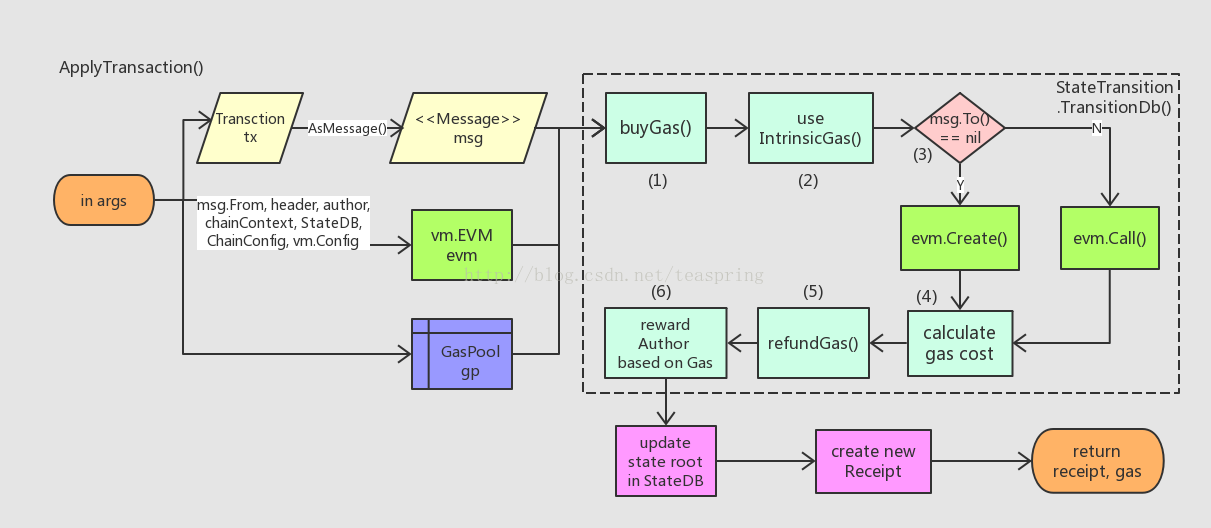
\includegraphics[scale=0.3]{applyTransaction.png}
	\caption{ApplyTransaction}
	\label{applyTransaction}
\end{figure}

\paragraph{GasPool}
GasPool类型是big.Int,在一个Block的处理过程中(即其所有tx的执行过程)中,GasPool的值能够告诉你,剩下还有多少Gas可以使用。
在每一个tx执行过程中,以太坊还设计了偿退(refund)环节,所refund的Gas数量也会加到这个GasPool里。

Process()函数的核心是一个for循环,它将Block里的所有tx遍历执行。具体的执行函数ApplyTransaction(),它每次执行tx,会返回一个收据(Receipt)对象。

ApplyTransaction()首先根据输入参数分别封装出一个Message对象和一个EVM对象,然后加上一个传入的GasPool类型变量,由TransitionDb()函数完成tx的执行,待TransitionDb()返回之后,创建一个收据Receipt对象,最后返回该Recetip对象,以及整个tx执行过程所消耗Gas数量。

GasPool对象是在一个Block执行开始时创建,并在该Block内所有tx的执行过程中共享,对于一个tx的执行可视为“全局”存储对象; Message由此次待执行的tx对象转化而来,并携带了解析出的tx的(转帐)转出方地址,属于待处理的数据对象;EVM 作为Ethereum世界里的虚拟机(Virtual Machine),作为此次tx的实际执行者,完成转帐和合约(Contract)的相关操作。

我们来细看下TransitioinDb()的执行过程(/core/state\_transition.go)。假设有StateTransition对象st,其成员变量initialGas表示初始可用Gas数量,gas表示即时可用Gas数量,初始值均为0,于是st.TransitionDb() 可由以下步骤展开:

\begin{itemize}
	\item 1. 购买Gas。首先从交易的(转帐)转出方账户扣除一笔Ether,费用等于tx.data.GasLimit * tx.data.Price;同时 st.initialGas = st.gas = tx.data.GasLimit;然后(GasPool) gp -= st.gas。

	\item 2. 计算tx的固有Gas消耗 - intrinsicGas。它分为两个部分,每一个tx预设的消耗量,这个消耗量还因tx是否含有(转帐)转入方地址而略有不同;以及针对tx.data.Payload的Gas消耗,Payload类型是[]byte,关于它的固有消耗依赖于[]byte中非0字节和0字节的长度。最终,st.gas -= intrinsicGas

	\item 3. EVM执行。如果交易的(转帐)转入方地址(tx.data.Recipient)为空,调用EVM的Create()函数;否则,调用Call()函数。无论哪个函数返回后,更新st.gas。

	\item 4. 计算本次执行交易的实际Gas消耗: requiredGas = st.initialGas - st.gas

	\item 5. 偿退Gas。它包括两个部分:首先将剩余st.gas 折算成Ether,归还给交易的(转帐)转出方账户;然后,基于实际消耗量requiredGas,系统提供一定的补偿,数量为refundGas。refundGas 所折算的Ether会被立即加在(转帐)转出方账户上,同时st.gas += refundGas,gp += st.gas,即剩余的Gas加上系统补偿的Gas,被一起归并进GasPool,供之后的交易执行使用。

	\item 6. 奖励所属区块的挖掘者:系统给所属区块的作者,亦即挖掘者账户,增加一笔金额,数额等于 st.data,Price * (st.initialGas - st.gas)。注意,这里的st.gas在步骤5中被加上了refundGas, 所以这笔奖励金所对应的Gas,其数量小于该交易实际消耗量requiredGas。
\end{itemize}
由上可见,除了步骤3中EVM 函数的执行,其他每个步骤都在围绕着Gas消耗量作文章(EVM 虚拟机的运行原理容后再述)。到这里,大家可以对Gas在以太坊系统里的作用有个初步概念,Gas就是Ethereum系统中的血液。

步骤5的偿退机制很有意思,设立它的目的何在?目前为止我只能理解它可以避免交易执行过程中过快消耗Gas,至于对其全面准确的理解尚需时日。

步骤6就更有趣了,正是这个奖励机制的存在,才会吸引社会上的矿工(miner)去卖力“挖矿”(mining)。越大的运算能力带来越多的的区块(交易)产出,矿工也就能通过该奖励机制赚取越多的以太币。

\begin{lstlisting}

/core/state_transition.go

// ApplyMessage computes the new state by applying the given message
// against the old state within the environment.
//
// ApplyMessage returns the bytes returned by any EVM execution (if it took place),
// the gas used (which includes gas refunds) and an error if it failed. An error always
// indicates a core error meaning that the message would always fail for that particular
// state and would never be accepted within a block.
func ApplyMessage(evm *vm.EVM, msg Message, gp *GasPool) ([]byte, uint64, bool, error) {
	return NewStateTransition(evm, msg, gp).TransitionDb()
}
\end{lstlisting}

\begin{lstlisting}

/core/types/receipt.go

// Receipt represents the results of a transaction.
type Receipt struct {
	// Consensus fields
	PostState         []byte `json:"root"`
	Status            uint64 `json:"status"`
	CumulativeGasUsed uint64 `json:"cumulativeGasUsed" gencodec:"required"`
	Bloom             Bloom  `json:"logsBloom"         gencodec:"required"`
	Logs              []*Log `json:"logs"              gencodec:"required"`

	// Implementation fields (don't reorder!)
	TxHash          common.Hash    `json:"transactionHash" gencodec:"required"`
	ContractAddress common.Address `json:"contractAddress"`
	GasUsed         uint64         `json:"gasUsed" gencodec:"required"`
}
\end{lstlisting}

\Emph{虚拟机内}

每个交易(Transaction)带有两部分内容需要执行:1. 转帐,由转出方地址向转入方地址转帐一笔以太币Ether; 2. 携带的[]byte类型成员变量Payload,其每一个byte都对应了一个单独虚拟机指令。这些内容都是由EVM(Ethereum Virtual Machine)对象来完成的。EVM 结构体是Ethereum虚拟机机制的核心,它与协同类的UML关系图如下:

\begin{figure}[ht]
	\centering
	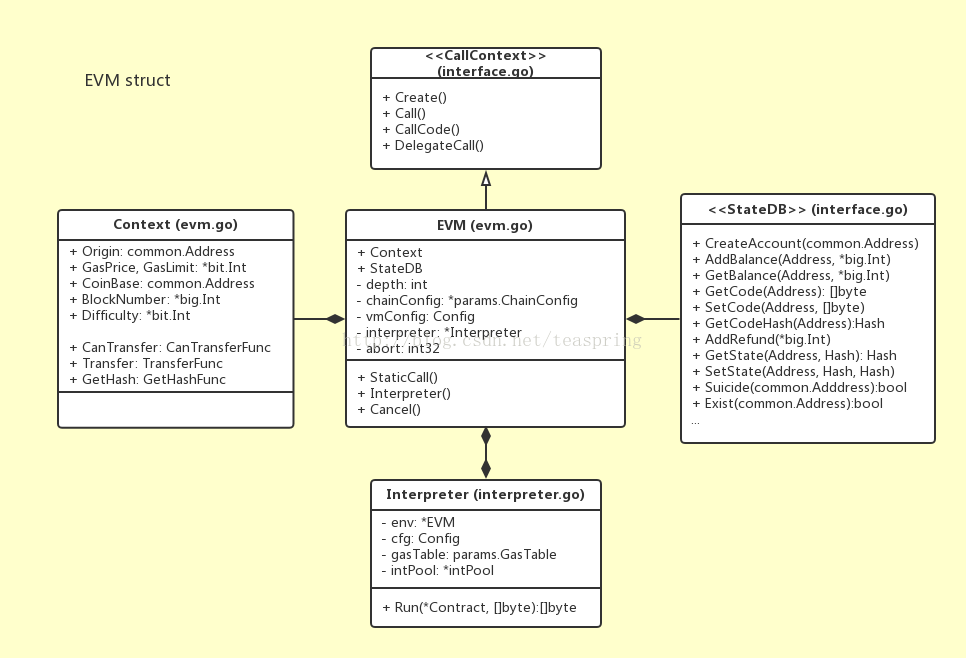
\includegraphics[scale=0.3]{evm.png}
	\caption{EVM}
	\label{evm}
\end{figure}

其中Context结构体分别携带了Transaction的信息(GasPrice, GasLimit),Block的信息(Number, Difficulty),以及转帐函数等,提供给EVM;StateDB 接口是针对state.StateDB 结构体设计的本地行为接口,可为EVM提供statedb的相关操作; Interpreter结构体作为解释器,用来解释执行EVM中合约(Contract)的指令(Code)。

注意,EVM 中定义的成员变量Context和StateDB, 仅仅声明了变量名而无类型,而变量名同时又是其类型名,在Golang中,这种方式意味着宗主结构体可以直接调用该成员变量的所有方法和成员变量,比如EVM调用Context中的Transfer()。

详情:https://blog.csdn.net/teaspring/article/details/75389151

\ifx\allfiles\undefined
\end{document}
\fi % 以太坊启动/区块和教育,合约和虚拟机

\ifx\allfiles\undefined
\documentclass[UTF8]{ctexart}
\title{以太坊挖共识算法与挖矿激励}
\author{邹远春}
\date{}
\usepackage{xeCJK}
\usepackage{graphicx}
\usepackage{listings}
\usepackage{verbatim}
\usepackage{graphicx}
\usepackage{xcolor}
\usepackage{listings}
\usepackage{amsmath}
\lstset{%
	breaklines=true,
	tabsize=2
}
\begin{document}
\maketitle
\newcommand\Emph{\textbf}
\else
\chapter{以太坊挖共识算法与挖矿激励}
\fi

本篇介绍了挖掘一个新区块在代码上的完整过程,从调用函数入口开始,沿调用过程一路向深,直至最终完成新区块授权/封印的共识算法,并对两种共识算法的设计思路和实现细节都进行了详细讲解。


\section{miner相关UML结构}

详情参考:[以太坊源代码分析]III. 挖矿和共识算法的奥秘 

https://blog.csdn.net/teaspring/article/details/78050274

\section{待挖掘区块需要组装}

在Ethereum 代码中,名为miner的包(package)负责向外提供一个“挖矿”得到的新区块,其主要结构体的UML关系图如下图所示:

\begin{figure}
	\centering
	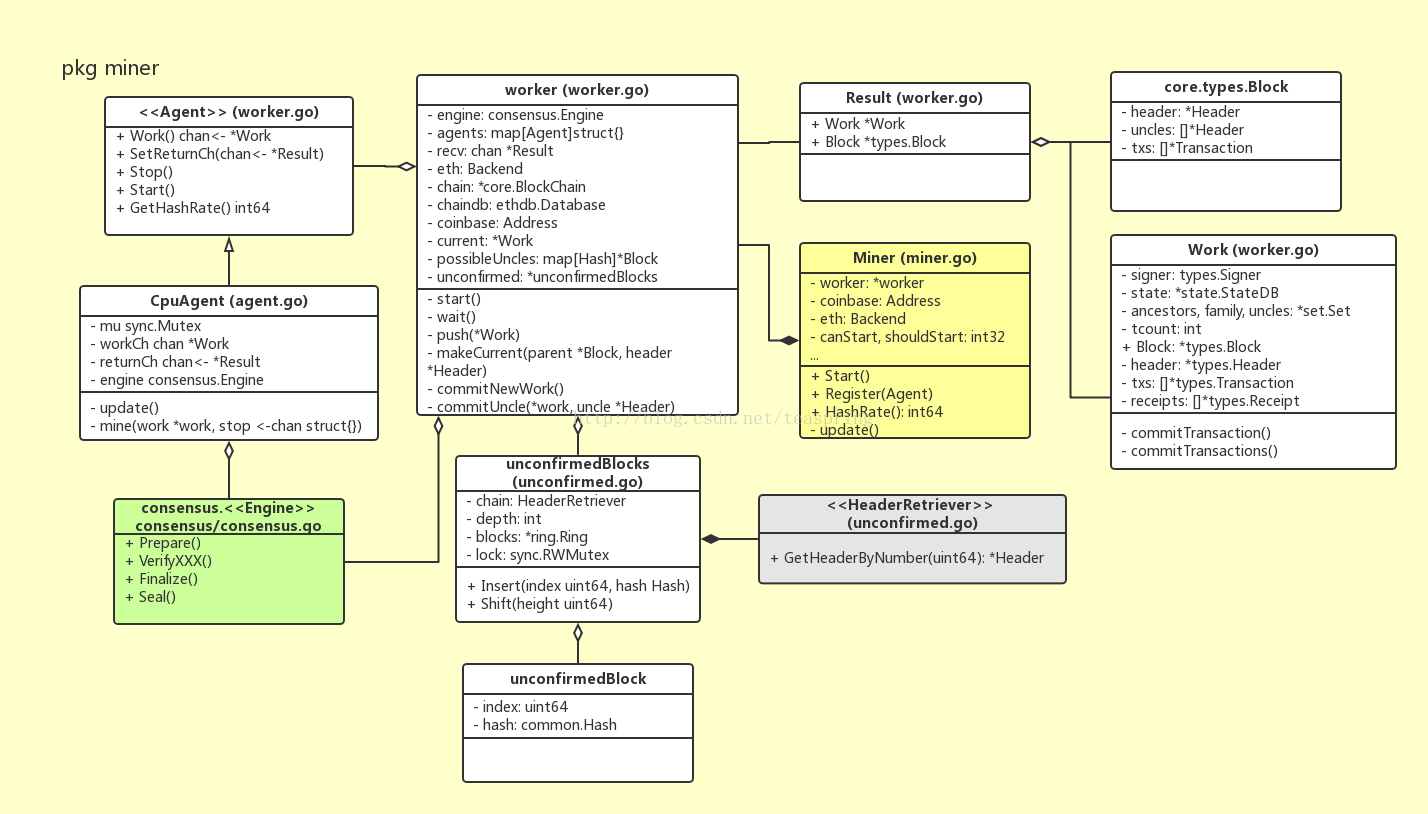
\includegraphics[scale=0.3]{miner.png}
	\caption{Miner}
	\label{miner}
\end{figure}

处于入口的类是Miner,它作为公共类型,向外暴露mine功能;它有一个worker类型的成员变量,负责管理mine过程;worker内部有一组Agent接口类型对象,每个Agent都可以完成单个区块的mine,目测这些Agent之间应该是竞争关系;Work结构体主要用以携带数据,被视为挖掘一个区块时所需的数据环境。

主要的数据传输发生在worker和它的Agent(们)之间:在合适的时候,worker把一个Work对象发送给每个Agent,然后任何一个Agent完成mine时,将一个经过授权确认的Block加上那个更新过的Work,组成一个Result对象发送回worker。

有意思的是<<Agent>>接口,尽管调用方worker内部声明了一个Agent数组,但目前只有一个实现类CpuAgent的对象会被加到该数组,可能这个Agent数组是为将来的扩展作的预留吧。CpuAgent通过全局的<<Engine>>对象,借助共识算法完成最终的区块授权。

另外,unconfirmedBlocks 也挺特别,它会以unconfirmedBlock的形式存储最近一些本地挖掘出的区块。在一段时间之后,根据区块的Number和Hash,再确定这些区块是否已经被收纳进主干链(canonical chain)里,以输出Log的方式来告知用户。

对于一个新区块被挖掘出的过程,代码实现上基本分为两个环节:一是组装出一个新区块,这个区块的数据基本完整,包括成员Header的部分属性,以及交易列表txs,和叔区块组uncles[],并且所有交易已经执行完毕,所有收据(Receipt)也已收集完毕,这部分主要由worker完成;二是填补该区块剩余的成员属性,比如Header.Difficulty等,并完成授权,这些工作是由Agent调用<Engine>接口实现体,利用共识算法来完成的。

\paragraph{新区块的组装流程}

挖掘新区块的流程入口在Miner里,略显奇葩的是,具体入口在Miner结构体的创建函数(避免称之为‘构造函数’)里。

\begin{figure}
	\centering
	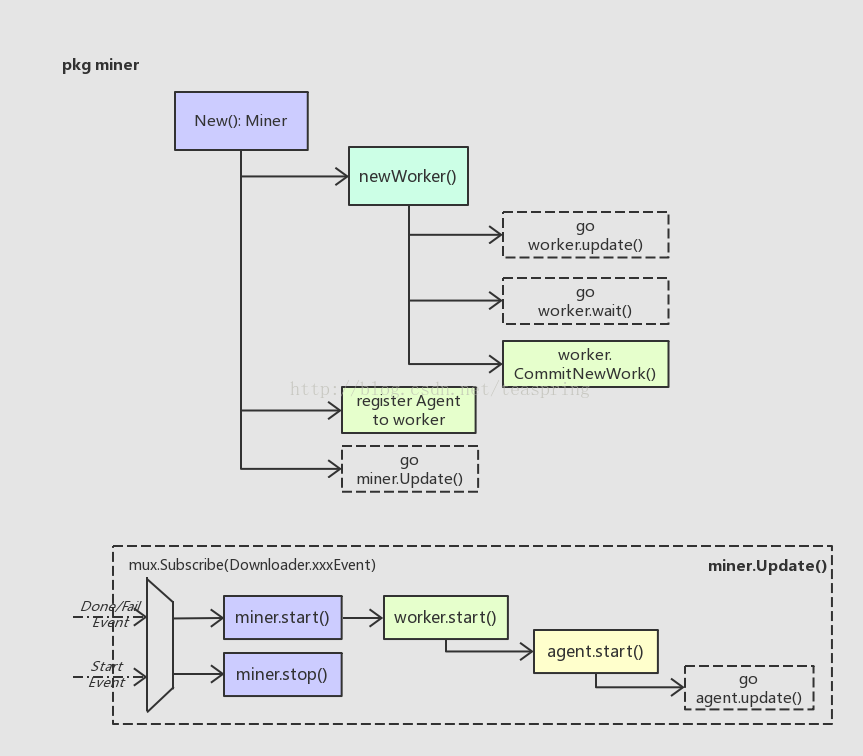
\includegraphics[scale=0.5]{newMiner.png}
	\caption{New Miner}
	\label{newMiner}
\end{figure}

\paragraph{Miner的函数}

\subparagraph{New()}

在New()里,针对新对象miner的各个成员变量初始化完成后,会紧跟着创建worker对象,然后将Agent对象登记给worker,最后用一个单独线程去运行miner.Update()函数;而worker的创建函数里也如法炮制,分别用单独线程去启动worker.updater()和wait();最后worker.CommitNewWork()会开始准备一个新区块所需的基本数据,如Header,Txs, Uncles等。注意此时Agent尚未启动。

\subparagraph{Update()}

这个update()会订阅(监听)几种事件,均跟Downloader相关。当收到Downloader的StartEvent时,意味者此时本节点正在从其他节点下载新区块,这时miner会立即停止进行中的挖掘工作,并继续监听;如果收到DoneEvent或FailEvent时,意味本节点的下载任务已结束-无论下载成功或失败-此时都可以开始挖掘新区块,并且此时会退出Downloader事件的监听。

从miner.Update()的逻辑可以看出,对于任何一个Ethereum网络中的节点来说,挖掘一个新区块和从其他节点下载、同步一个新区块,根本是相互冲突的。这样的规定,保证了在某个节点上,一个新区块只可能有一种来源,这可以大大降低可能出现的区块冲突,并避免全网中计算资源的浪费。

\subparagraph{worker的函数}
这里我们主要关注worker.updater()和wait()

\begin{figure}
	\centering
	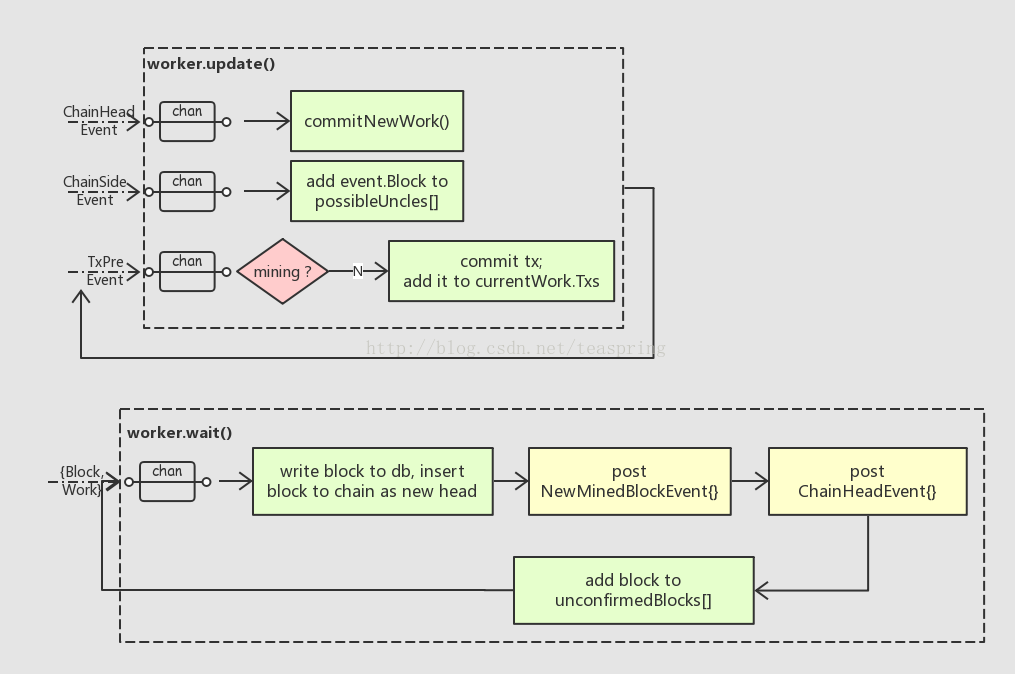
\includegraphics[scale=0.4]{worker.png}
	\caption{worker}
	\label{worker}
\end{figure}

\subparagraph{update()}

worker.update()分别监听ChainHeadEvent,ChainSideEvent,TxPreEvent几个事件,每个事件会触发worker不同的反应。ChainHeadEvent是指区块链中已经加入了一个新的区块作为整个链的链头,这时worker的回应是立即开始准备挖掘下一个新区块(也是够忙的);ChainSideEvent指区块链中加入了一个新区块作为当前链头的旁支,worker会把这个区块收纳进possibleUncles[]数组,作为下一个挖掘新区块可能的Uncle之一;TxPreEvent是TxPool对象发出的,指的是一个新的交易tx被加入了TxPool,这时如果worker没有处于挖掘中,那么就去执行这个tx,并把它收纳进Work.txs数组,为下次挖掘新区块备用。

需要稍稍注意的是,ChainHeadEvent并不一定是外部源发出。由于worker对象有个成员变量chain(eth.BlockChain),所以当worker自己完成挖掘一个新区块,并把它写入数据库,加进区块链里成为新的链头时,worker自己也可以调用chain发出一个ChainHeadEvent,从而被worker.update()函数监听到,进入下一次区块挖掘。

\subparagraph{wait()}

worker.wait()会在一个channel处一直等待Agent完成挖掘发送回来的新Block和Work对象。这个Block会被写入数据库,加入本地的区块链试图成为最新的链头。注意,此时区块中的所有交易,假设都已经被执行过了,所以这里的操作,不会再去执行这些交易对象。

当这一切都完成,worker就会发送一条事件(NewMinedBlockEvent{}),等于通告天下:我挖出了一个新区块!这样监听到该事件的其他节点,就会根据自身的状况,来决定是否接受这个新区块成为全网中公认的区块链新的链头。至于这个公认过程如何实现,就属于共识算法的范畴了。

\subparagraph{commitNewWork()}

commitNewWork()会在worker内部多处被调用,注意它每次都是被直接调用,并没有以goroutine的方式启动。commitNewWork()内部使用sync.Mutex对全部操作做了隔离。这个函数的基本逻辑如下:

\begin{itemize}

\item 准备新区块的时间属性Header.Time,一般均等于系统当前时间,不过要确保父区块的时间(parentBlock.Time())要早于新区块的时间,父区块当然来自当前区块链的链头了。

\item 创建新区块的Header对象,其各属性中:Num可确定(父区块Num +1);Time可确定;ParentHash可确定;其余诸如Difficulty,GasLimit等,均留待之后共识算法中确定。

\item 调用Engine.Prepare()函数,完成Header对象的准备。

\item 根据新区块的位置(Number),查看它是否处于DAO硬分叉的影响范围内,如果是,则赋值予header.Extra。

\item 根据已有的Header对象,创建一个新的Work对象,并用其更新worker.current成员变量。

\item 如果配置信息中支持硬分叉,在Work对象的StateDB里应用硬分叉。

\item 准备新区块的交易列表,来源是TxPool中那些最近加入的tx,并执行这些交易。

\item 准备新区块的叔区块uncles[],来源是worker.possibleUncles[],而possibleUncles[]中的每个区块都从事件ChainSideEvent中搜集得到。注意叔区块最多有两个。

\item 调用Engine.Finalize()函数,对新区块“定型”,填充上Header.Root, TxHash, ReceiptHash, UncleHash等几个属性。

\item 如果上一个区块(即旧的链头区块)处于unconfirmedBlocks中,意味着它也是由本节点挖掘出来的,尝试去验证它已经被吸纳进主干链中。

\item 把创建的Work对象,通过channel发送给每一个登记过的Agent,进行后续的挖掘。

\end{itemize}

以上步骤中,4和6都是仅仅在该区块配置中支持DAO硬分叉,并且该区块的位置正好处于DAO硬分叉影响范围内时才会发生;其他步骤是普遍性的。commitNewWork()完成了待挖掘区块的组装,block.Header创建完毕,交易数组txs,叔区块Uncles[]都已取得,并且由于所有交易被执行完毕,相应的Receipt[]也已获得。万事俱备,可以交给Agent进行‘挖掘’了。

\paragraph{CpuAgent的函数}

CpuAgent中与mine相关的函数,主要是update()和mine():

\begin{figure}
	\centering
	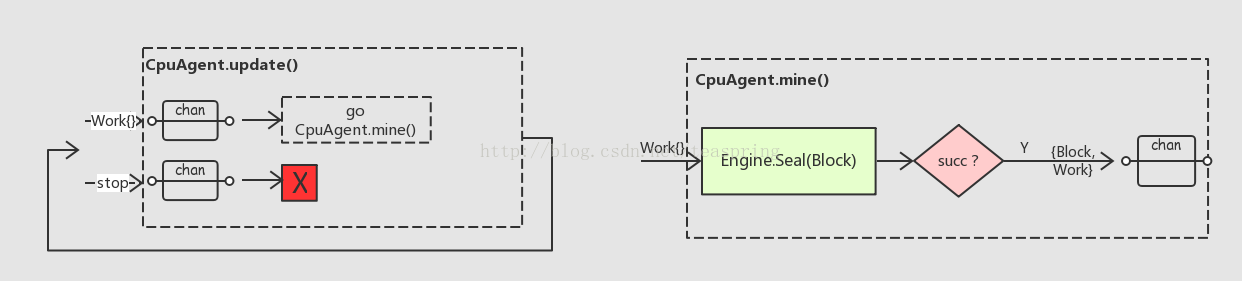
\includegraphics[scale=0.3]{cpuagent.png}
	\caption{Cpu Agent}
	\label{cpuAgent}
\end{figure}

\subparagraph{CpuAgent.update()}就是worker.commitNewWork()结束后发出Work对象的会一直监听相关channel,如果收到Work对象(显然由worker.commitNewWork()结束后发出),就启动mine()函数;如果收到停止(mine)的消息,就退出一切相关操作。

\subparagraph{CpuAgent.mine()}会直接调用Engine.Seal()函数,利用Engine实现体的共识算法对传入的Block进行最终的授权,如果成功,就将Block同Work一起通过channel发还给worker,那边worker.wait()会接收并处理。

显然,这两个函数都没做什么实质性工作,它们只是负责调用<Engine>接口实现体,待授权完成后将区块数据发送回worker。挖掘出一个区块的真正奥妙全在Engine实现体所代表的共识算法里。

\section{共识算法完成挖掘}

共识算法族对外暴露的是Engine接口,其有两种实现体,分别是基于运算能力的Ethash算法和基于“同行”认证的的Clique算法。

\begin{figure}
	\centering
	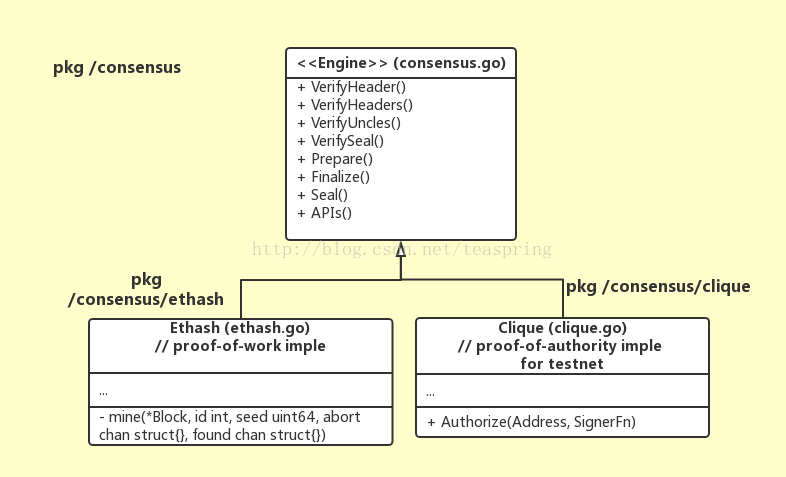
\includegraphics[scale=0.5]{consensus.png}
	\caption{consensus}
	\label{consensus}
\end{figure}

在Engine接口的声明函数中,VerifyHeader(),VerifyHeaders(),VerifyUncles()用来验证区块相应数据成员是否合理合规,可否放入区块;Prepare()函数往往在Header创建时调用,用来对Header.Difficulty等属性赋值;Finalize()函数在区块区块的数据成员都已具备时被调用,比如叔区块(uncles)已经具备,全部交易Transactions已经执行完毕,全部收据(Receipt[])也已收集完毕,此时Finalize()会最终生成Root,TxHash,UncleHash,ReceiptHash等成员。

而Seal()和VerifySeal()是Engine接口所有函数中最重要的。Seal()函数可对一个调用过Finalize()的区块进行授权或封印,并将封印过程产生的一些值赋予区块中剩余尚未赋值的成员(Header.Nonce, Header.MixDigest)。Seal()成功时返回的区块全部成员齐整,可视为一个正常区块,可被广播到整个网络中,也可以被插入区块链等。所以,对于挖掘一个新区块来说,所有相关代码里Engine.Seal()是其中最重要,也是最复杂的一步。VerifySeal()函数基于跟Seal()完全一样的算法原理,通过验证区块的某些属性(Header.Nonce,Header.MixDigest等)是否正确,来确定该区块是否已经经过Seal操作。

在两种共识算法的实现中,Ethash是产品环境下以太坊真正使用的共识算法,Clique主要针对以太坊的测试网络运作,两种共识算法的差异,主要体现在Seal()的实现上。

\paragraph{Ethash共识算法}

Ethash算法又被称为Proof-of-Work(PoW),是基于运算能力的授权/封印过程。Ethash实现的Seal()函数,其基本原理可简单表示成以下公式:

\begin{center}
$RAND(h, n) <= M / d$
\end{center}

这里M表示一个极大的数,比如$2^{256}-1$;d表示Header成员Difficulty。RAND()是一个概念函数,它代表了一系列复杂的运算,并最终产生一个类似随机的数。这个函数包括两个基本入参:h是Header的哈希值(Header.HashNoNonce()),n表示Header成员Nonce。整个关系式可以大致理解为,在最大不超过M的范围内,以某个方式试图找到一个数,如果这个数符合条件(<=M/d),那么就认为Seal()成功。

我们可以先定性的验证一个\Emph{推论:d的大小对整个关系式的影响}。假设h,n均不变,如果d变大,则M/d变小,那么对于RAND()生成一个满足该条件的数值,显然其概率是下降的,即意味着难度将加大。考虑到以上变量的含义,当Header.Difficulty逐渐变大时,这个对应区块被挖掘出的难度(恰为Difficulty本义)也在缓慢增大,挖掘所需时间也在增长,所以上述推论是合理的。

\subparagraph{mine()函数}
Ethash.Seal()函数实现中,会以多线程(goroutine)的方式并行调用mine()函数,线程个数等于Ethash.threads;如果Ethash.threads被设为0,则Ethash选择以本地CPU中的总核数作为开启线程的个数。

\begin{lstlisting}

/* consensus/ethash/sealer.go */
func (ethash *Ethash) mine(block *Block, id int, seed uint64, abort chan struct{}, found chan *Block) {
    var (
        header = block.Header()
        hash   = header.HashNoNonce().Bytes()
        target = new(big.Int).Div(maxUint256, header.Difficulty)
        number = header.Number.Uint64()
        dataset = ethash.dataset(number)
        nonce  = seed
    )
    for {
        select {
        case <-abort:
            ...; return
        default:
            digest, result := hashimotoFull(dataset, hash, nonce) // compute the PoW value of this nonce
            if new(big.Int).SetBytes(result).Cmp(target) <= 0 { // x.Cmp(y) <= 0 means x <= y
                header = types.CopyHeader(header)
                header.Nonce = types.EncodeNonce(nonce)
                header.MixDigest = common.BytesToHash(digest)
                found<- block.WithSeal(header)
                return
            }
        }
        nonce++
    }
}

\end{lstlisting}


以上代码就是mine()函数的主要业务逻辑。入参@id是线程编号,用来发送log告知上层;函数内部首先定义一组局部变量,包括之后调用hashimotoFull()时传入的hash、nonce、巨大的辅助数组dataset,以及结果比较的target;然后是一个无限循环,每次调用hashimotoFull()进行一系列复杂运算,一旦它的返回值符合条件,就复制Header对象(深度拷贝),并赋值Nonce、MixDigest属性,返回经过授权的区块。注意到在每次循环运算时,nonce还会自增+1,使得每次循环中的计算都各不相同。

这里hashimotoFull()函数通过调用hashimoto()函数完成运算,而同时还有另外一个类似的函数hashimoLight()函数。

\begin{lstlisting}

func hashimotoFull(dataset []uint32, hash []byte, nonce uint64) ([]byte, []byte) {
    lookup := func(index uint32) []uint32 {
        offset := index * hashWords
        return dataset[offset : offset+hashWords]
    }
    return hashimoto(hash, nonce, uint64(len(dataset))*4, lookup)
}
func hashimotoLight(size uint64, cache []uint32, hash []byte, nonce uint64) ([]byte, []byte) {
    lookup := func(index uint32) []uint32 {
        rawData := generateDatasetItem(cache, index, keccak512)
        data := make([]uint32, len(rawData)/4)
        for i := 0; i < len(data); i++ {
            data[i] = binary.LittleEndian.Uint32(rawData[i*4:])
        }
        return data
    }
    return hashimoto(hash, nonce, size, lookup)
}

\end{lstlisting}

以上两个函数,最终都调用了hashimoto()。它们的差别,在于各自调用hashimoto()函数的入参@size uint 和 @lookup func()不同。相比于Light(),Full()函数调用的size更大,以及一个从更大数组中获取数据的查询函数lookup()。\Emph{hashimotoFull()函数是被Seal()调用的},而hashimotoLight()是为VerifySeal()准备的。

这里的lookup()函数其实很重要,它其实是一个以非线性表查找方式进行的哈希函数! 这种哈希函数的性能不仅取决于查找的逻辑,更多的依赖于所查找的表格的数据规模大小。lookup()会以函数型参数的形式传递给hashimoto()

\Emph{核心的运算函数hashimoto()}

最终为Ethash共识算法的Seal过程执行运算任务的是hashimoto()函数,它的函数类型如下:

\begin{lstlisting}
// consensus/ethash/algorithm.go
func hashimoto(hash []byte, nonce uint64, size uint64, lookup(index uint32) []uint32) (digest []byte, result []byte)
\end{lstlisting}

hashimoto()函数的入参包括:区块哈希值@hash, 区块nonce成员@nonce,和非线性表查找的哈希函数lookup(),及其所查找的非线性表格的容量@size。返回值digest和result,都是32 bytes长的字节串。
hashimoto()的逻辑比较复杂,包含了多次、多种哈希运算。下面尝试从其中数据结构变化的角度来简单描述之:


\begin{figure}
	\centering
	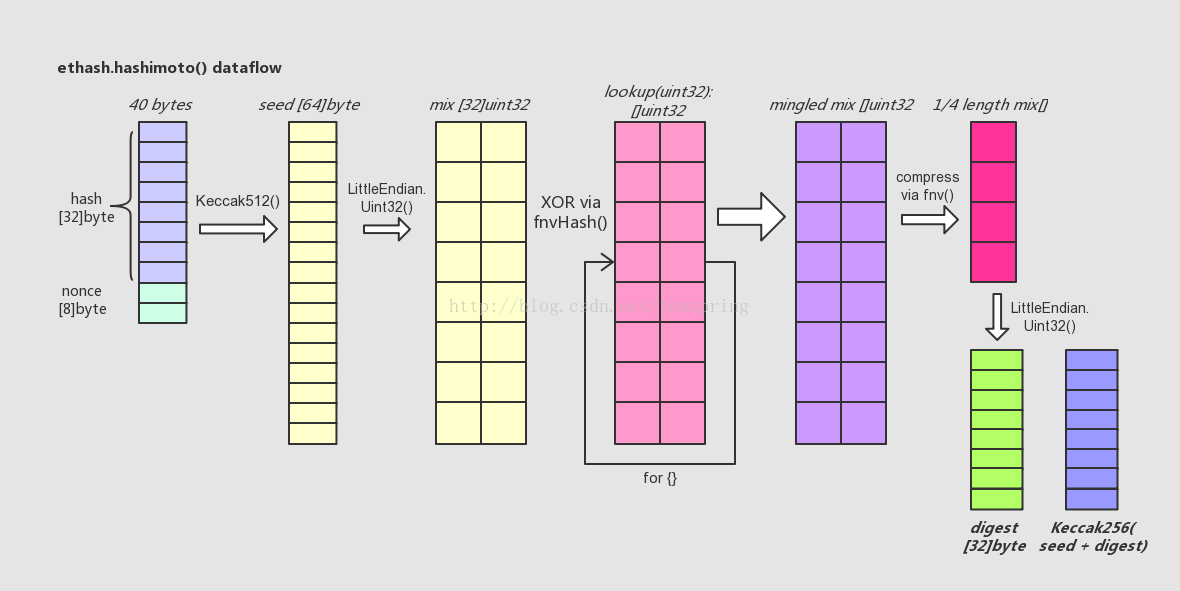
\includegraphics[scale=0.3]{hashimoto.png}
	\caption{hashimoto}
	\label{hashimoto}
\end{figure}


简单介绍一下上图所代表的代码流程:

\begin{itemize}

\item 首先,hashimoto()函数将入参@hash和@nonce合并成一个40 bytes长的数组,取它的SHA-512哈希值取名seed,长度为64 bytes。

\item 然后,将seed[]转化成以uint32为元素的数组mix[],注意一个uint32数等于4 bytes,故而seed[]只能转化成16个uint32数,而mix[]数组长度32,所以此时mix[]数组前后各半是等值的。

\item 接着,lookup()函数登场。用一个循环,不断调用lookup()从外部数据集中取出uint32元素类型数组,向mix[]数组中混入未知的数据。循环的次数可用参数调节,目前设为64次。每次循环中,变化生成参数index,从而使得每次调用lookup()函数取出的数组都各不相同。这里混入数据的方式是一种类似向量“异或”的操作,来自于FNV算法。

\item 待混淆数据完成后,得到一个基本上面目全非的mix[],长度为32的uint32数组。这时,将其折叠(压缩)成一个长度缩小成原长1/4的uint32数组,折叠的操作方法还是来自FNV算法。

\item 最后,将折叠后的mix[]由长度为8的uint32型数组直接转化成一个长度32的byte数组,这就是返回值@digest;同时将之前的seed[]数组与digest合并再取一次SHA-256哈希值,得到的长度32的byte数组,即返回值@result。
\end{itemize}

最终经过一系列多次、多种的哈希运算,hashimoto()返回两个长度均为32的byte数组 - digest[]和result[]。回忆一下ethash.mine()函数中,对于hashimotoFull()的两个返回值,会直接以big.int整型数形式比较result和target;如果符合要求,则将digest取SHA3-256的哈希值(256 bits),并存于Header.MixDigest中,待以后Ethash.VerifySeal()可以加以验证。

\Emph{以非线性表查找方式进行的哈希运算}

上述hashimoto()函数中,函数型入参lookup()其实表示的是一次以非线性表查找方式进行的哈希运算,lookup()以入参为key,从所关联的数据集中按照定义好的一段逻辑取出64 bytes长的数据作为hash value并返回,注意返回值以uint32的形式则相应变成16个uint32长。返回的数据会在hashimoto()函数被其他的哈希运算所使用。

以非线性表的查找方式进行的哈希运算(hashing by nonlinear table lookup),属于众多哈希函数中的一种实现,在Ethash算法的核心环节有大量使用,所使用到的非线性表被定义成两种结构体,分别叫cache{}和dataset{}。二者的差异主要是表格的规模和调用场景:dataset{}中的数据规模更加巨大,从而会被hashimotoFull()调用从而服务于Ethash.Seal();cache{}内含数据规模相对较小,会被hashimotoLight()调用并服务于Ethash.VerifySeal()。

\begin{figure}
	\centering
	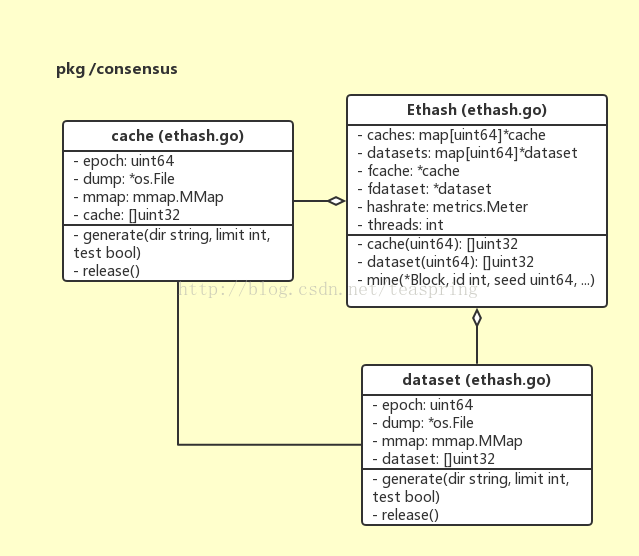
\includegraphics[scale=0.5]{ethash.png}
	\caption{ethash}
	\label{ethash}
\end{figure}


以cache{}的结构体声明为例,成员cache就是实际使用的一块内存Buffer,mmap是内存映射对象,dump是该内存buffer存储于磁盘空间的文件对象,epoch是共享这个cache{}对象的一组区块的序号。从上述UML图来看,cache和dataset的结构体声明基本一样,这也暗示了它们无论是原理还是行为都极为相似。

\Emph{cache\{\}对象的生成}


dataset{}和cache{}的生成过程很类似,都是通过内存映射的方式读/写磁盘文件。

\begin{figure}
	\centering
	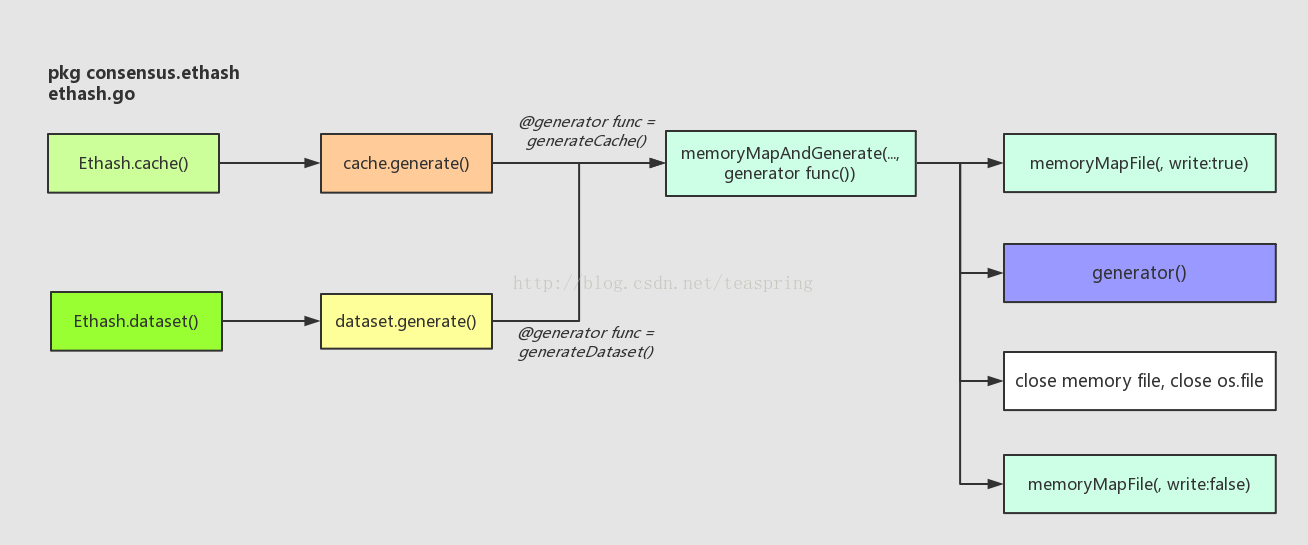
\includegraphics[scale=0.3]{cache.png}
	\caption{cache}
	\label{cache}
\end{figure}

以cache{}为例,Ethash.cache(uint64)会确保该区块所用到的cache{}对象已经创建,它的入参是区块的Number,用Number/epochLength可以得到该区块所对应的epoch号。epochLength被定义成常量30000,意味着每连续30000个区块共享一个cache{}对象。

有意思的是内存映射相关的函数,memoryMapAndGenerate()会首先调用memoryMapFile()生成一个文件并映射到内存中的一个数组,并调用传入的函数型参数generator() 进行数据的填入,于是这个内存数组以及所映射的磁盘文件就同时变得十分巨大,注意此时传入memoryMapFile()的文件操作权限是可写的。然后再关闭所有文件操作符,调用memoryMapFile()重新打开这个磁盘文件并映射到内存的一个数组,注意此时的文件操作权限是只读的。可见这组函数的coding很精细。

Ethash中分别用一个map结构来存放不同epoch对应的cache对象和dataset对象,缓存成员fcache和fdataset,用以提前创建cache{}和dataset{}对象以避免下次使用时再花费时间。

我们以cache{}为例,看看cache.generate()方法的具体逻辑:

\begin{figure}
	\centering
	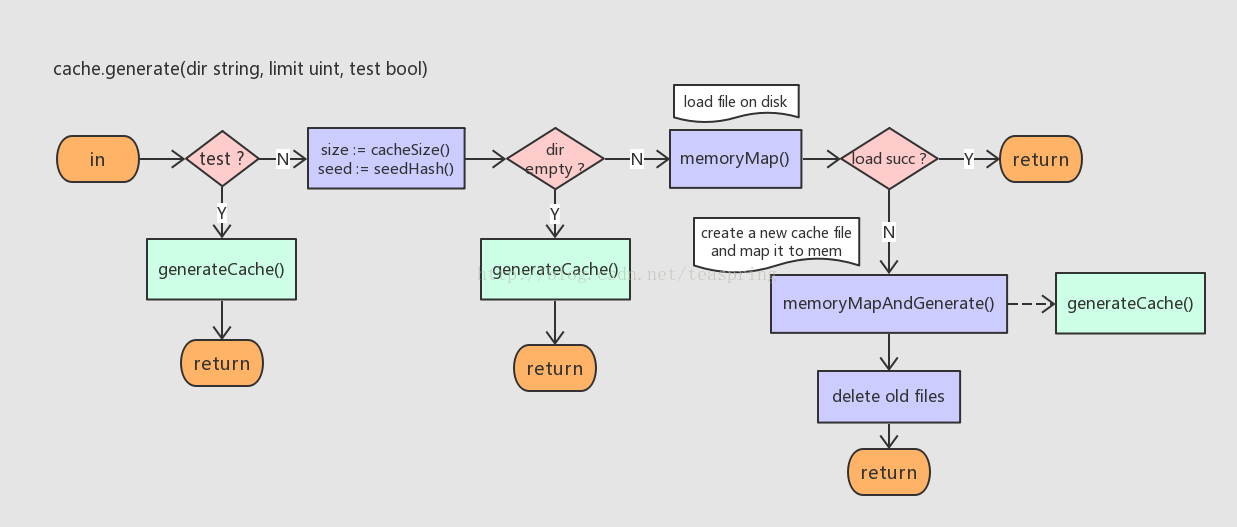
\includegraphics[scale=0.3]{cache_generate.png}
	\caption{cache generate}
	\label{cacheGenerate}
\end{figure}

上图是cache.generate()方法的基本流程:如果是测试用途,则不必考虑磁盘文件,直接调用generateCache()创建buffer;如果文件夹为空,那也没法拼接出文件路径,同样直接调用generateCache()创建buffer;然后根据拼接出的文件路径,先尝试读取磁盘上已有文件,如果成功,说明文件已存在并可使用;如果文件不存在,那只好创建一个新文件,定义文件容量,然后利用内存映射将其导入内存。很明显,直接为cache{]创建buffer的generateCache()函数是这里的核心操作,包括memoryMapAndGenerate()方法,都将generateCache()作为一个函数型参数引入操作的。

\Emph{参数size的生成}

参数size是生成buffer的容量,它在上述cache.generate()中生成。

\begin{lstlisting}

size = cacheSize(epoch * epochLength +1)
...
func cacheSize(block uint64) uint64 {
    epoch := int(block / epochLength)
    if epoch < len(cacheSizes) {
        return cacheSizes[epoch]
    }
    size := uint64(cacheInitBytes + cacheGrowthBytes * uint64(epoch) - hashBytes)
    for !(size/hashBytes).ProbablyPrime(1) {
        size -= 2 * hashBytes
    }
    return size
}

\end{lstlisting}

上述就是生成size的代码,cacheSize()的入参虽然是跟区块Number相关,但实际上对于处于同一epoch组的区块来说效果是一样的,每组个数epochLength。Ethash在代码里预先定义了一个数组cacheSizes[],存放了前2048个epoch组所用到的cache size。如果当前区块的epoch处于这个范围内,则取用之;若没有,则以下列公式赋初始值。

\begin{center}
$size = cacheInitBytes + cacheGrowthBytes * epoch - hashBytes$
\end{center}

这里$cacheInitBytes = 2^{24}$,$cacheGrowthBytes = 2^{17}$,hashBytes = 64,可见size的取值有多么巨大了。注意到cacheSize()中在对size赋值后还要不断调整,保证最终size是个质数,这是出于密码学的需要。

粗略计算一下size的取值范围,$size = 2^{24} + 2^{17} * epoch$,由于$epoch > 2048 = 2^{11}$,所以$size  > 2^{28}$,生成的buffer至少有256MB,而这还仅仅是VerifySeal()使用的cache{},Seal()使用的dataset{}还要大的多,可见这些数据集有多么庞大了。

\Emph{参数seed[]的生成}

参数seed是generateCache()中对buffer进行哈希运算的种子数据,它也在cache.generate()函数中生成。

\begin{lstlisting}

seed := seedHash(epoch * epochLength +1)
...
func seedHash(block uint64) []byte {
    seed := make([]byte, 32)
    if block < epochLength { // epochLength = 30000
        return seed
    }
    keccak256 := makeHasher(sha3.NewKeccak256())
    for i := 0; i < int(block/epochLength); i++ {
        keccak256(seed, seed)
    }
    return seed
}
type hasher func(dest []byte, data []byte)
func makeHasher(h hash.Hash) hasher {
    return func(dest []byte, data []byte) {
        h.Write(data)
        h.Sum(dest[:0])
        h.Reset()
    }
}


\end{lstlisting}

上述seedHash()函数用来生成所需的seed[]数组,它的长度32bytes,与common.Address类型长度相同。makeHasher()函数利用入参的哈希函数接口生成一个哈希函数,这里用了SHA3-256哈希函数。注意seedHash()中利用生成的哈希函数keccak256()对seed[]做的原地哈希,而原地哈希运算的次数跟当前区块所处的epoch序号有关,所以每个不同的cache{}所用到的seed[]也是完全不同的,这个不同通过更多次的哈希运算来实现。


\Emph{generateCache()函数}


generateCache()函数在给定种子数组seed[]的情况下,对固定容量的一块buffer进行一系列操作,使得buffer的数值分布变得随机、无规律可循,最终buffer作为cache{}中的数组(非线性表)返回,还可作为数据源帮助生成dataset{}。generateCache()函数主体分两部分,首先用SHA3-512哈希函数作为哈希生成器(hasher),对buffer数组分段(每次64bytes)进行哈希化,然后利用StrictMemoryHardFunction中的RandMemoHash算法对buffer再进行处理。这个RandMemoHash算法来自2014年密码学方向的一篇学术论文,有兴趣的朋友可以搜搜看。

\Emph{内存映射}

由于Ethash(PoW)算法中用到的随机数据集cache{}和dataset{}过于庞大,将其以文件形式存储在磁盘上就显得很有必要。同样由于这些文件过于庞大,使用时又需要一次性整体读入内存(因为对其的使用是随意截取其中的一段数据),使用内存映射可以大大减轻I/O负担。cache{}和dataset{}结构体中,均有一个mmap对象用以操作内存映射,以及一个系统文件对象dump,对应于打开的磁盘文件。



\Emph{Ethash算法总结:}

回看一下Ethash共识算法最基本的形态,如果把整个result[]的生成过程视作那个概念上的函数RAND(),则如何能更加随机,分布更加均匀的生成数组,关系到整个Ethash算法的安全性。毕竟如果result[]生成过程存在被破译的途径,那么必然有方法可以更快地找到符合条件的数组,通过更快的挖掘出区块,在整个以太坊系统中逐渐占据主导。所以Ethash共识算法应用了非常复杂的一系列运算,包含了多次、多种不同的哈希函数运算:

\begin{itemize}

\item 大量使用SHA3哈希函数,包括256-bit和512-bit形式的,用它们来对数据(组)作哈希运算,或者充当其他更复杂哈希计算的某个原型 -- 比如调用makeHasher()。而SHA3哈希函数,是一种典型的可应对长度变化的输入数据的哈希函数,输出结果长度统一(可指定256bits或512bits)。

\item lookup()函数提供了非线性表格查找方式的哈希函数,相关联的dataset{}和cache{}规模巨大,其中数据的生成/填充过程中也大量使用哈希函数。

\item 在一些计算过程中,有意将[]byte数组转化为uint32或uint64整型数进行操作(比如XOR,以及类XOR的FNV()函数)。因为理论证实,在32位或64位CPU机器上,以32位/64位整型数进行操作时,速度更快。
\end{itemize}

\paragraph{Clique共识算法}
Clique算法又称Proof-of-Authortiy(PoA),它实现的Seal()其实是一个标准的数字签名加密过程,可由下列公式表示:

\begin{center}
$n = F(pr, h)$
\end{center}

其中F()是数字签名函数,n是生成的数字签名,pr是公钥,h是被加密的内容。具体到Clique应用中,n是一个65 bytes长的字符串,pr是一个common.Address类型的(长度20 bytes)地址,h是一个common.Hash类型(32 bytes)的哈希值,而签名算法F(),目前采用的正是\Emph{椭圆曲线数字签名算法}(ECDSA)。

没错,就是这个被用来生成交易(Transaction)对象的数字签名的ECDSA。在Clique的实现中,这里用作公钥的Address类型地址有一个限制,它必须是已认证的(authorized)。所以Clique.Seal()函数的基本逻辑就是:有一个Address类型地址打算用作数字签名的公钥(不是区块的作者地址Coinbase);如果它是已认证的,则执行指定的数字签名算法。而其中涉及到的动态管理所有认证地址的机制,才是Clique算法(PoA)的精髓。

\Emph{基于投票的地址认证机制}

首先了解一下Clique的认证机制authorization所包括的一些设定:

\begin{itemize}

\item 所有的地址(Address类型)分为两类,分别是经过认证的,和未经过认证的。

\item 已认证地址(authorized)可以变成未认证的,反之亦然。不过这些变化都必须通过投票机制完成。

\item 一张投票包括:投票方地址,被投票地址,和被投票地址的新认证状态。有效投票必须满足:被投票地址的新认证地址与其现状相反。

\item 任意地值A只能给地址B投一张票
\end{itemize}

这些设定理解起来并不困难,把这里的地址替换成平常生活中的普通个体,这就是个很普通的投票制度。Clique算法中的投票系统的巧妙之处在于,每张投票并不是某个投票方主动“投”出来的,而是随机组合出来的。

想了解更多细节免不了要深入一些代码,下图是Clique算法中用到的一些结构体:

\begin{figure}
	\centering
	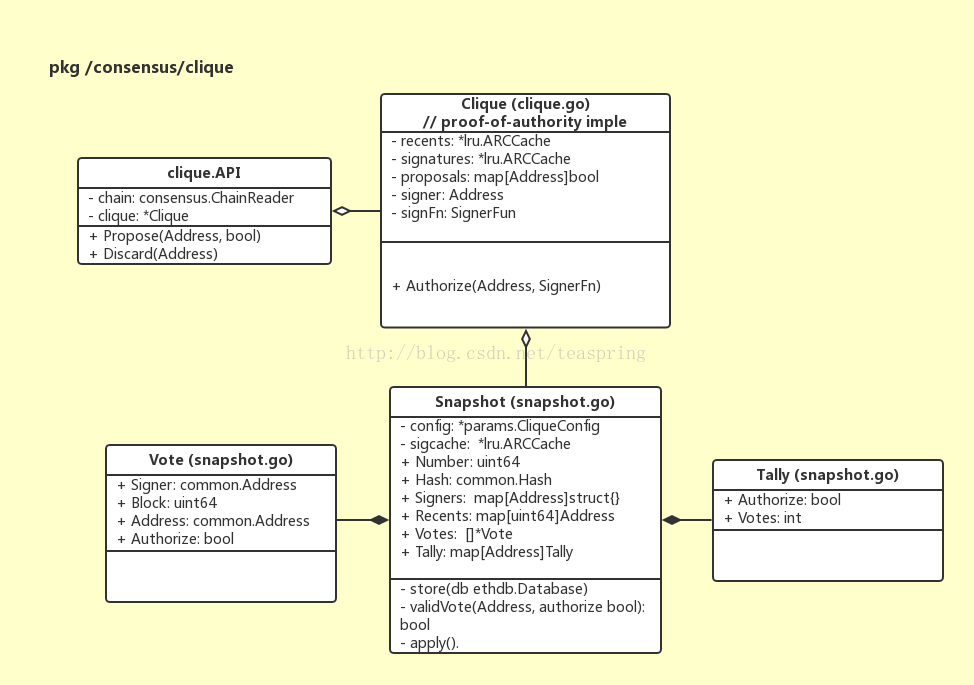
\includegraphics[scale=0.4]{clique.png}
	\caption{clique}
	\label{clique}
\end{figure}

Clique结构体实现了共识算法接口Engine的所有方法,它可对区块作Seal操作。它的成员signFn正是数字签名生成函数,signer用作数字签名的公钥,这两成员均由Authorize()函数进行赋值。它还有一个map类型成员proposals,用来存放所有的不记名投票,即每张投票只带有被投票地址和投票内容(新认证状态),由于是map类型,显然这里的proposals存放的是内容不同的不记名投票。API结构体对外提供方法,可以向Clique的成员变量proposals插入或删除投票。

Snapshot结构体用来动态管理认证地址列表,在这里认证地址是分批次存储和更新的,一个Snapshot对象,存放的是以区块为时序的所有认证地址的"快照"。Snapshot的成员Number和Hash,正是区块Block的标志属性;成员Signers存储所有已认证地址。

一个Vote对象表示一张记名投票。Tally结构体用来记录投票数据,即某个(被投票)地址总共被投了多少票,新认证状态是什么。Snapshot中用map型变量Tally来管理所有Tally对象数据,map的key是被投票地址,所以Snapshot.Tally记录了被投票地址的投票次数。另外Snapshot还有一个Vote对象数组,记录所有投票数据。

\Emph{新区块的Coinbase是一个随机的被投票地址}

Engine接口的Prepare()方法,约定在Header创建后调用,用以对Header的一些成员变量赋值,比如作者地址Coinbase。在Clique算法中,新区块的Coinbase来自于proposals中的某个被投票地址。

\begin{figure}
	\centering
	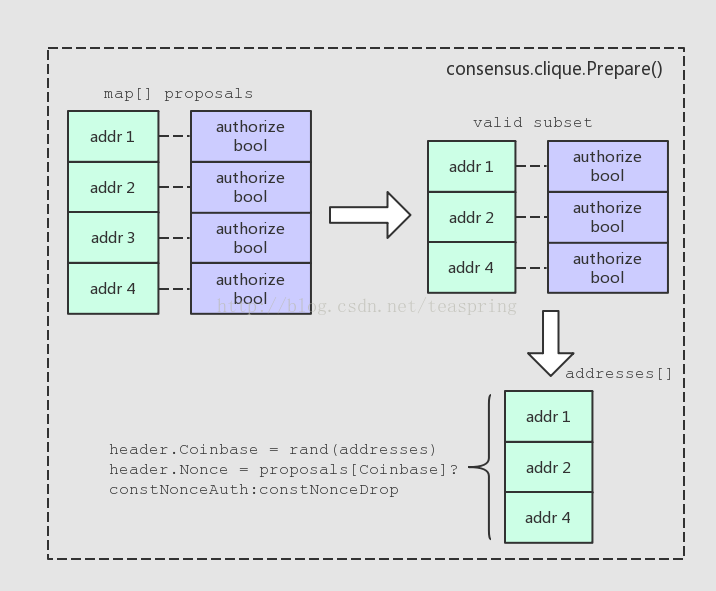
\includegraphics[scale=0.5]{clique_coinbase.png}
	\caption{clique coinbase}
	\label{cliqueCoinbase}
\end{figure}

上图解释了Clique.Prepare()方法中的部分逻辑。首先从proposals中筛选出有效的不记名投票,要么是已认证地址变为未认证,要么反过来;然后获取有效的被投票地址列表,从中随机选取一个地址作为该区块的Coinbase,与之相应的投票内容则被区块的Nonce属性携带。而新区块的Coinbase会在之后的更新认证地址环节,被当作一次投票的被投票地址。

ps,Ethash算法中,新区块的Coinbase地址可是异常重要的,因为它会作为新区块的作者地址,被系统奖励或补偿以太币。但Clique算法中就完全不同了,由于工作在测试网络中,每个帐号地址获得多少以太币没有实际意义,所以这里的Coinbase任意赋值倒也无妨。

\Emph{添加记名投票并更新认证地址列表}

管理所有认证地址的结构体是Snapshot,具体到更新认证地址列表的方法是apply()。它的基本流程如下图:

\begin{figure}
	\centering
	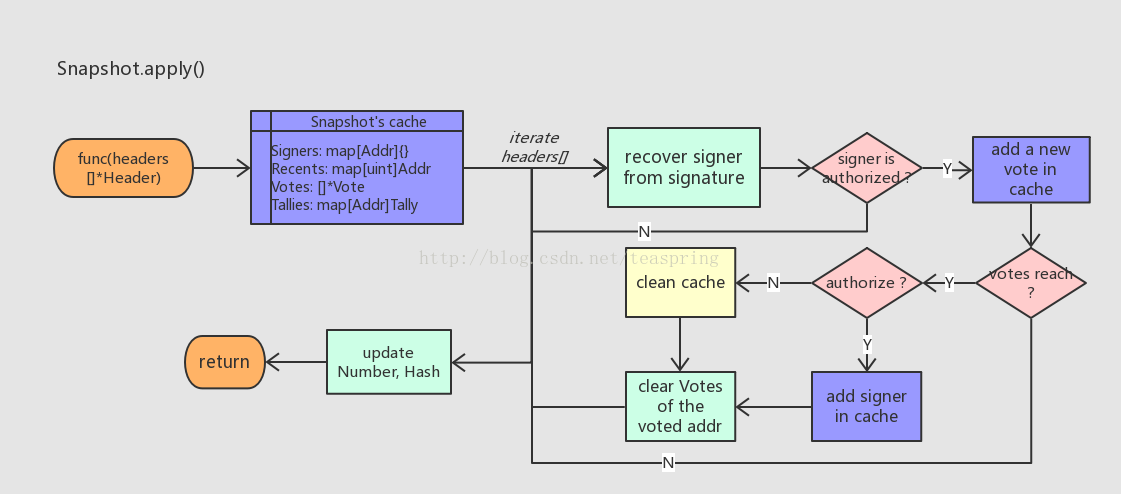
\includegraphics[scale=0.3]{snapshot.png}
	\caption{Snapshot}
	\label{snapshot}
\end{figure}

重温一下Snapshot结构体内声明的一组缓存成员变量:

\Emph{Signers}是全部已认证地址集合,注意这里用map类型来提供Set的行为。

\Emph{Recents}用来记录最近担当过数字签名算法的signer的地址,通过它Snapshot可以控制某个地址不会频繁的担当signer。更重要的是,由于signer地址会充当记名投票的投票方,所以Recents可以避免某些地址频繁的充当投票方!Recents中map类型的key是区块Number值。

\Emph{Votes}记录了所有尚未失效的记名投票;Tallies记录了所有被投票地址(voted)目前的(被)投票次数。

Snapshot.apply()函数的入参是一组Header对象,它们来自区块主链上按从旧到新顺序排列的一组区块,并且严格衔接在Snapshot当前状态(成员Number,Hash)之后。注意,这些区块都是当前“待挖掘”新区块的祖先,所以它们的成员属性都是已经确定的。apply()方法的主要部分是迭代处理每个Header对象,处理单个Header的流程如下:

\begin{itemize}

\item 首先从数字签名中恢复出签名所用公钥,转化为common.Address类型,作为signer地址。数字签名(signagure)长度65 bytes,存放在Header.Extra[]的末尾。

\item 如果signer地址是尚未认证的,则直接退出本次迭代;如果是已认证的,则记名投票+1。所以一个父区块可添加一张记名投票,signer作为投票方地址,Header.Coinbase作为被投票地址,投票内容authorized可由Header.Nonce取值确定。

\item 更新投票统计信息。如果被投票地址的总投票次数达到已认证地址个数的一半,则通过之。

\item 该被投票地址的认证状态立即被更改,根据是何种更改,相应的更新缓存数据,并删除过时的投票信息。

\end{itemize}

在所有Header对象都被处理完后,Snapshot内部的Number,Hash值会被更新,表明当前Snapshot快照结构已经更新到哪个区块了。

Snapshot.apply()方法在Clique.Seal()中被调用,具体位于运行数字签名算法之前,以保证即将充当公钥的地址可以用最新的认证地址列表加以验证。



综上所述,Clique算法在投票制度的安全性设计上完善了诸多细节:

\begin{itemize}

\item 外部参与不记名投票的方式是通过API.Propose(),Discard()来操作Clique.proposals。由于proposals是map类型,所以每个投票地址(map的key)在proposals中只能存在一份,这样就杜绝了外部通过恶意操作Clique.proposals来影响不记名投票数据的企图。

\item 所有认证地址的动态更新,由一张张记名投票累计作用影响。而每张记名投票的投票方地址和投票内容(不记名投票),是以毫不相关、近乎随机的方式组合起来的。所以,理论上几乎不存在外部恶意调用代码从而操纵记名投票数据的可能。同时,通过一些内部缓存(Snapshot.Recents),避免了某些signer地址过于频繁的充当投票方地址。

\end{itemize}

虽然Clique共识算法并非作用在产品环境,但它依然很精巧的设计了完整的基于投票的选拔制度,很好的践行了"去中心化"宗旨。这对于其他类型共识算法的设计,提供了一个不错的样本。

\Emph{小结}

本篇介绍了挖掘一个新区块在代码上的完整过程,从调用函数入口开始,沿调用过程一路向深,直至最终完成新区块授权/封印的共识算法,并对两种共识算法的设计思路和实现细节都进行了详细讲解。

\begin{itemize}

\item 一般所说的“挖掘一个新区块”其实包括两部分,第一阶段组装出新区块的所有数据成员,包括交易列表txs、叔区块uncles等,并且所有交易都已经执行完毕,各帐号状态更新完毕;第二阶段对该区块进行授勋/封印(Seal),没有成功Seal的区块不能被广播给其他节点。第二阶段所消耗的运算资源,远超第一阶段。

\item Seal过程由共识算法(consensus algorithm)族完成,包括Ethash算法和Clique算法两种实现。前者是产品环境下真实采用的,后者是针对测试网络(testnet)使用的。Seal()函数并不会增加或修改区块中任何跟有效数据有关的部分,它的目的是通过一系列复杂的步骤,或计算或公认,选拔出能够出产新区块的个体。

\item \Emph{Ethash算法(PoW)基于运算能力来筛选出挖掘区块的获胜者},运算过程中使用了大量、多次、多种的哈希函数,通过极高的计算资源消耗,来限制某些节点通过超常规的计算能力轻易形成“中心化”倾向。

\item \Emph{Clique算法(PoA)利用数字签名算法完成Seal操作},不过签名所用公钥,同时也是common.Address类型的地址必须是已认证的。所有认证地址基于特殊的投票地址进行动态管理,记名投票由不记名投票和投票方地址随机组合而成,杜绝重复的不记名投票,严格限制外部代码恶意操纵投票数据

\item 在实践“去中心化”方面,以太坊还在区块结构中增加了叔区块(uncles)成员以加大计算资源的消耗,并通过在交易执行环节对叔区块作者(挖掘者)的奖励,以收益机制来调动网络中各节点运算资源分布更加均匀。

\end{itemize}

\ifx\allfiles\undefined
\end{document}
\fi % 以太坊共识算法

\include{angiosperms}

\appendix

\chapter{APG分类系统的科名}

内容附录内容附录内容附录内容附录内容附录内容附录内容附录内容附录内容附录内容附录内容附录内容附录内容附录内容附录内容附录内容附录内容附录内容文内容正文内容正文内容正文\index{内容}

内容附录内容附录内容附录内容附录内容附录内容附录内容附录内容附录内容附录内容附录内容附录内容附录内容附录内容附录内容附录内容附录内容附录内容附录内容附录内容附录内容正文内容正文\cite{DK1}.

\renewcommand\indexname{索~~引}
\printindex
\addcontentsline{toc}{chapter}{索~引}

\backmatter

\addcontentsline{toc}{chapter}{参考文献}

\begin{thebibliography}{参考文献}
\bibitem[Knuth1 et al. 1997]{DK1} D. Knuth, T.A.O.C.P. , Vol. 1, Addison-Wesley, 1997.
\bibitem[Knuth2]{DK2} D. Knuth, T.A.O.C.P. , Vol. 2, Addison-Wesley, 1997.
\bibitem[TONG YH 2014]{TONG} TONG YH, PANG KS, XIAN NH, 2014. Carpinus insularis (Betulaceae), A new species from Hong Kong [J]. J Trop Subtrop Bot, 22(2): 121-124. [童毅华, 彭权森, 夏念和,2014. 香港桦木科一新种——香港鹅耳枥 [J]. 热带亚热带植物学报,22(2):121-124.]
\bibitem[XIA NH 2008]{XIA} XIA NH, DENG YF, YIP KL, 2008. Syzygium impressum (Myrtaceae), A new species from Hong Kong [J]. J Trop Subtrop Bot, 16(1):19-22. [夏念和,邓云飞,叶国梁,2008. 香港桃金娘科一新种-凹脉赤楠 [J].热带亚热带植物学报,16(1):19-22.]
\end{thebibliography}

\chapter{后~~记}

后记内容后记内容后记内容后记内容后记内容后记内容后记内容后记内容后记内容后记内容后记内容后记内容后记内容后记内容后记内容后记内容后记内容后记内容后记内容后记内容后记内容后记内容后记内容后记内容后记内容后记内容后记内容后记内容后记内容后记内容后记内容后记内容后记内容后记内容后记内容后记内容后记内容后记内容后记内容后记内容后记内容后记内容后记内容后记内容后记内容后记内容后记内容后记内容后记内容后记内容后记内容后记内容后记内容后记内容后记内容后记内容后记内容后记内容后记内容后记内容后记内容后记内容后记内容后记内容后记内容

\begin{flushright}
作~~者~~~~~~~~~

2018年1月~~~~~
\end{flushright}

\end{document}
